% --------------------------- Implementation ---------------------------------

\pagebreak

\section{Implementation}
\subsection{Features From RM}
\noindent
For the initial prototype development, a subset of the requirements from the Requirement Matrix (RM) was carefully selected to focus on implementing core functionalities and demonstrating proof of concept. The selection was based on a combination of high-priority functional requirements that form the backbone of the system, ensuring that critical features are built and validated before expanding the scope.

The requirements chosen for the prototype primarily involve data preprocessing, model training, and evaluation processes. These requirements were selected because they are fundamental to the project's success, ensuring that the data pipeline and model implementation work seamlessly together. This subset of features lays the groundwork for later integration with additional components and more complex functionality.

The filtered part of the RM focuses on the following high-priority requirements: data cleaning and feature extraction, training of machine learning models, and evaluation of model performance using standard metrics. These requirements were identified as crucial because they directly impact the system's ability to handle data, learn patterns, and provide meaningful outputs. Without successfully implementing these core features, the overall effectiveness of the solution would be significantly reduced.

Furthermore, these selected features align with the project’s goals and provide a clear pathway for incremental development. By narrowing down the requirements to these foundational aspects, the development team can ensure that the prototype is not only functional but also extensible, providing a robust framework for future enhancements.

\begin{figure}[h!]  
    \centering
    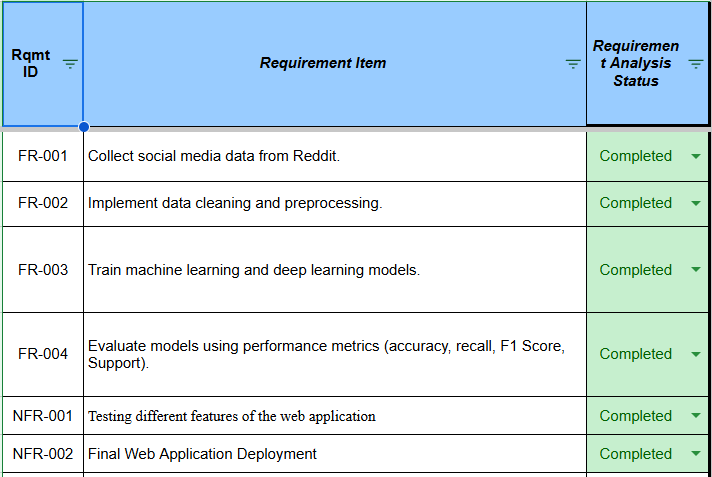
\includegraphics[width=0.7\textwidth]{Images/RM_part_for_implementation.png}  
    \caption{Features from Requirement Matrix}
    \label{Features from Requirement Matrix}  % Label for referencing the figure
\end{figure}

\subsection{Code Details and Output}

\subsubsection{Data Collection}

\begin{tcolorbox}[colback=gray!5!white, colframe=gray!80!black, boxrule=0.5pt, title=Collecting Reddit Posts]
    \begin{lstlisting}[language=Python]
import praw
import pandas as pd
import time
# Initialize Reddit API
reddit = praw.Reddit(client_id='YOUR_CLIENT_ID',
                        client_secret='YOUR_CLIENT_SECRET',
                        user_agent='Mental Health Classifier')
# Define subreddits and post types
subreddits = {'normal': ['news', 'AskReddit'], 
                'depression': ['depression'], 
                'ptsd': ['PTSD'], 
                'anxiety': ['Anxiety'], 
                'bipolar': ['BipolarReddit']}
post_types = ['hot', 'new', 'top']
posts_per_type = 100
# Collect and save posts
data = []
for label, subs in subreddits.items():
    for sub in subs:
        for post_type in post_types:
            posts = getattr(reddit.subreddit(sub), post_type)(limit=posts_per_type)
            for post in posts:
                data.append([post.title + " " + post.selftext, label])
            time.sleep(1)
df = pd.DataFrame(data, columns=['text', 'label'])
df.to_csv(f'{label}_dataset.csv', index=False)
    \end{lstlisting}
    \end{tcolorbox}
    
    \begin{figure}[h!]  
        \centering
        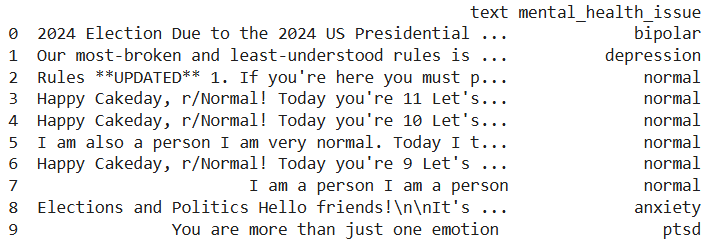
\includegraphics[width=0.9\textwidth]{Images/Dataset.png}  
        \caption{Obtained Dataset}
        \label{LSTMROC711}  % Label for referencing the figure
    \end{figure}


\begin{tcolorbox}[colback=gray!5!white, colframe=gray!80!black, boxrule=0.5pt, title=Combining Collected Datasets]
\begin{lstlisting}[language=Python]
import pandas as pd
from sklearn.utils import shuffle

# Load datasets
bipolar_df = pd.read_csv("bipolar_dataset.csv")
depression_df = pd.read_csv("depression_dataset.csv")
normal_df = pd.read_csv("normal_dataset.csv")
anxiety_df = pd.read_csv("anxiety_dataset.csv")
ptsd_df = pd.read_csv("ptsd_dataset.csv")

# Minimum length for balanced classes
min_length = min(len(bipolar_df), len(depression_df), len(normal_df) // 6, len(anxiety_df), len(ptsd_df))

# Create balanced pattern
pattern_data = []
for i in range(min_length):
    pattern_data.extend([bipolar_df.iloc[i], depression_df.iloc[i]] +
                        normal_df.iloc[i*6:(i+1)*6].to_dict('records') +
                        [anxiety_df.iloc[i], ptsd_df.iloc[i]])

pattern_df = pd.DataFrame(pattern_data)
remaining_data = shuffle(pd.concat([bipolar_df[min_length:], depression_df[min_length:], 
                                    normal_df[min_length*6:], anxiety_df[min_length:], ptsd_df[min_length:]]))

final_df = pd.concat([pattern_df, remaining_data]).reset_index(drop=True)
final_df.to_csv("mental_health_combined.csv", index=False)
\end{lstlisting}
\end{tcolorbox}
    
\noindent
The first code snippet collects Reddit posts by connecting to specific subreddits associated with various mental health topics. Using the Reddit API, posts are retrieved from `hot`, `new`, and `top` categories for each mental health type, including general subreddits (for the "normal" category). Each post’s title and content are combined, labeled, and saved into separate CSV files. The second code snippet merges these CSV files to form a combined dataset. It creates a balanced sample by selecting the minimum number of rows across each category and organizes the data in a structured pattern. Remaining rows are shuffled and appended, producing a final dataset suitable for machine learning applications in mental health classification.
    

% ----- adding subreddit info ------

\begin{figure}[h!]  
    \centering
    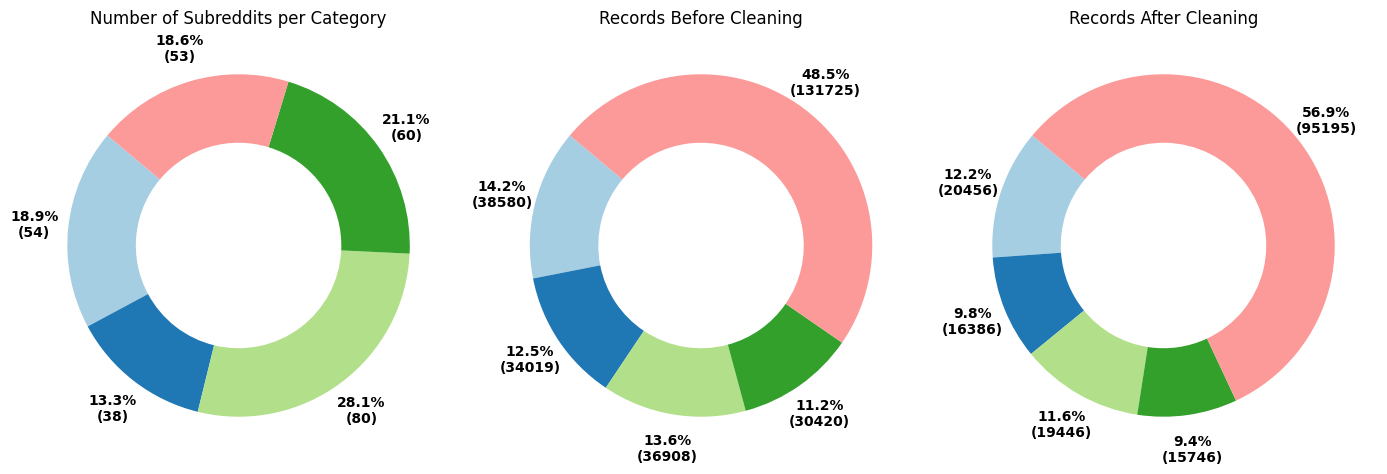
\includegraphics[width=1.0\textwidth]{Images/Data Collection Graph.png}  
    \caption{Collected Data Statistics}
    \label{LSTMROC7uyiut11}  % Label for referencing the figure
\end{figure}

\noindent
The dataset for mental health classification was compiled from various subreddit communities. Initially, the dataset contained records from 54 subreddits for anxiety, 38 for PTSD, 80 for depression, 60 for bipolar disorder, and 53 for normal mental states. Before data cleaning, the records totaled 38580 for anxiety, 34019 for PTSD, 36908 for depression, 30420 for bipolar, and 131725 for normal, reflecting the distribution of raw data. After applying data cleaning techniques to ensure quality and relevance, the record counts were reduced to 20456 for anxiety, 16386 for PTSD, 19446 for depression, 15746 for bipolar, and 95195 for normal. A subset of this cleaned dataset containing 18596 records was used for further processing and analysis.

\vspace{1em}

\noindent
Given the large size of the original dataset, training and testing the model on the entire dataset would require significant computational resources, including memory and processing power. Such constraints can lead to prolonged training times and potentially infeasible execution on standard hardware. By using a subset of the cleaned dataset, we can significantly reduce the computational load while maintaining a representative sample of the data. This approach strikes a balance between efficiency and performance, enabling the development and evaluation of models in a more manageable and resource-friendly manner. Moreover, working with a subset ensures faster experimentation and fine-tuning cycles, which is crucial for iterative improvement in machine learning workflows.

\pagebreak

\subsubsection{Data Preprocessing}

\begin{tcolorbox}[colback=gray!5!white, colframe=gray!80!black, boxrule=0.5pt, title=Text Preprocessing]
    \begin{lstlisting}[language=Python]
import pandas as pd
import re
from sklearn.feature_extraction.text import TfidfVectorizer
from nltk.corpus import stopwords
from nltk.tokenize import word_tokenize
import nltk

# Download stopwords (if you haven't already)
nltk.download('stopwords')
nltk.download('punkt')

# Load the dataset
df = pd.read_csv('mental_health.csv')

# 1. Handling Missing Values
df.dropna(subset=['text'], inplace=True)

# 2. Removing duplicates (if any)
df.drop_duplicates(subset=['text'], inplace=True)

# 3. Text Preprocessing
negative_words = {"not", "no", "nor", "never", "nothing", "nowhere", "neither", "cannot", "n't", "without", "barely", "hardly", "scarcely"}

def clean_text(text):
    text = re.sub(r'http\S+', '', text)  # Remove URLs
    text = re.sub(r'@\w+', '', text)  # Remove mentions (@username)
    text = re.sub(r'[^a-zA-Z\s]', '', text)  # Remove special characters, numbers, and punctuations
    text = text.lower()  # Convert text to lowercase
    tokens = word_tokenize(text)  # Tokenize the text
    tokens = [word for word in tokens if word not in stopwords.words('english') or word in negative_words]  # Remove stopwords, but keep negative words
    clean_text = ' '.join(tokens)  # Join the tokens back into a single string
    return clean_text

df['cleaned_text'] = df['text'].apply(clean_text)  # Apply the cleaning function to the 'text' column

\end{lstlisting}
\end{tcolorbox}

\begin{tcolorbox}[colback=gray!5!white, colframe=gray!80!black, boxrule=0.5pt, title=Text Preprocessing]
\begin{lstlisting}[language=Python]
# 4. Feature Extraction using TF-IDF Vectorization
vectorizer = TfidfVectorizer(max_features=10000)  # Adjust the max_features
X = vectorizer.fit_transform(df['cleaned_text'])  # Fit and transform the cleaned text data
X_df = pd.DataFrame(X.toarray(), columns=vectorizer.get_feature_names_out())  # Convert the result to a DataFrame for easier understanding

# Save the preprocessed dataset (optional)
df.to_csv('preprocessed_mental_health.csv', index=False)
    \end{lstlisting}
\end{tcolorbox}

\noindent
The code snippet above demonstrates the preprocessing steps for a mental health dataset. It handles missing values and duplicates in the text data, performs text cleaning by removing URLs, mentions, and special characters, and applies tokenization. The cleaned text is then vectorized using TF-IDF to convert the textual data into a format suitable for machine learning models. Finally, the preprocessed dataset is saved as a new CSV file for future use in classification tasks.

\begin{figure}[h!]  
    \centering
    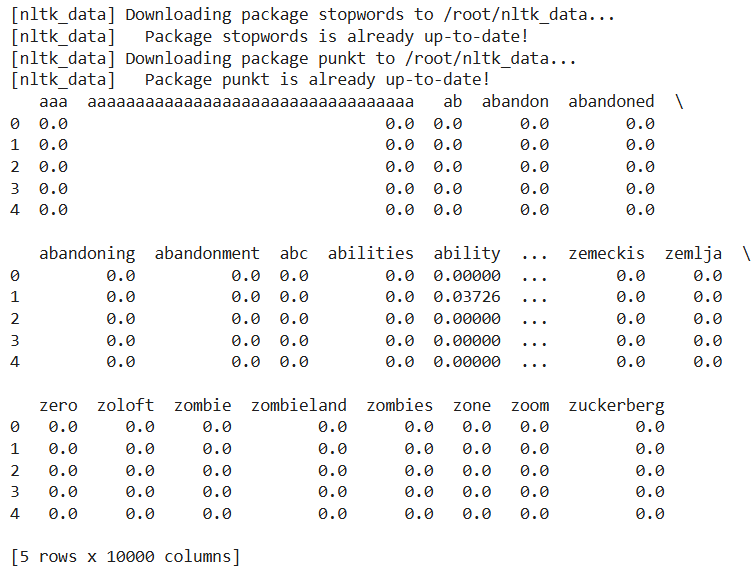
\includegraphics[width=0.9\textwidth]{Images/Data Cleaning and Preprocessing.png}  
    \caption{Data Collection and Preprocessing}
    \label{Data Collection and Preprocessing}  % Label for referencing the figure
\end{figure}

% ------------ OTHER VECTORIZATIONS

\subsubsection{Vectorization Technqiues}

% Bag of Words
\begin{tcolorbox}[colback=gray!5!white, colframe=gray!80!black, boxrule=0.5pt, title=Bag of Words]
\begin{lstlisting}[language=Python]
from sklearn.feature_extraction.text import CountVectorizer

# Initialize the CountVectorizer and fit/transform the cleaned text
vectorizer = CountVectorizer()
X = vectorizer.fit_transform(dataset['cleaned_text'])
\end{lstlisting}
\end{tcolorbox}

\noindent
Bag of Words (BoW) converts text into a matrix of word counts. Each unique word in the corpus becomes a feature, and the value is the word's frequency in the document, ignoring grammar and word order.

% TF-IDF
\begin{tcolorbox}[colback=gray!5!white, colframe=gray!80!black, boxrule=0.5pt, title=TF-IDF]
\begin{lstlisting}[language=Python]
from sklearn.feature_extraction.text import TfidfVectorizer

# Initialize the TfidfVectorizer and fit/transform the cleaned text
TFIDFvectorizer = TfidfVectorizer()
X = TFIDFvectorizer.fit_transform(dataset['cleaned_text'])
\end{lstlisting}
\end{tcolorbox}

\noindent
Term Frequency-Inverse Document Frequency (TF-IDF) weighs words by their importance in a corpus. Common words receive lower weights, while rare words are assigned higher values, capturing their significance in the document.

% N-Gram
\begin{tcolorbox}[colback=gray!5!white, colframe=gray!80!black, boxrule=0.5pt, title=N-Gram]
\begin{lstlisting}[language=Python]
from sklearn.feature_extraction.text import CountVectorizer

# Initialize the CountVectorizer with n-grams (e.g., bi-grams and tri-grams)
vectorizer = CountVectorizer(ngram_range=(1, 3))
X = vectorizer.fit_transform(dataset['cleaned_text'])
\end{lstlisting}
\end{tcolorbox}
    
\noindent
N-Grams capture contiguous sequences of words to preserve some context. For example, bigrams (2-grams) capture pairs of words like "machine learning," and trigrams (3-grams) capture sequences like "natural language processing."

% LIWC
\begin{tcolorbox}[colback=gray!5!white, colframe=gray!80!black, boxrule=0.5pt, title=LIWC (Empath)]
\begin{lstlisting}[language=Python]
from empath import Empath

# Initialize Empath
lexicon = Empath()

# Function to get Empath features
def get_empath_features(text):
    analysis = lexicon.analyze(text, normalize=True)  # Normalize for proportions
    return analysis

# Generate Empath features for each text
empath_features = dataset['cleaned_text'].apply(get_empath_features)

# Convert Empath features to a DataFrame
X = pd.DataFrame(empath_features.tolist())
\end{lstlisting}
\end{tcolorbox}

\noindent
LIWC (Linguistic Inquiry and Word Count) analyzes text by categorizing words into meaningful psychological or social dimensions. Empath is a Python library that replicates this functionality with customizable lexicons. Empath is a Python-based natural language processing tool inspired by LIWC (Linguistic Inquiry and Word Count), designed to analyze text and categorize words into psychologically meaningful dimensions such as emotions, cognitive processes, and social themes. This tool is particularly valuable for extracting semantic features that capture the psychological and emotional aspects of textual data, making it ideal for applications in sentiment analysis, mental health studies, and psycholinguistics. By matching words in the text to predefined categories, Empath assigns a proportional representation to each category, indicating the relative frequency of words that belong to it. In the provided code, an \texttt{Empath} object is initialized, which serves as the base for analyzing text against the predefined lexicons. A function named \texttt{get\_empath\_features} is defined to process individual texts from the dataset. This function leverages the \texttt{analyze} method of the \texttt{Empath} object to compute the distribution of words across various categories. The \texttt{normalize=True} parameter ensures that the output represents proportions rather than raw counts, making the results more interpretable and comparable across texts of varying lengths. The function is applied to each piece of cleaned text in the dataset, producing a structured output where each text is represented as a dictionary. Each key in this dictionary corresponds to an Empath category, and the associated value indicates the proportion of words from the text that fall into that category. The list of dictionaries generated through this process is then converted into a DataFrame, where each column represents a category and each row corresponds to a document in the dataset. This transformation allows the extracted features to be seamlessly integrated into machine learning pipelines, where they can serve as predictors for tasks like sentiment analysis, mental health classification.

% Word2Vec
\begin{tcolorbox}[colback=gray!5!white, colframe=gray!80!black, boxrule=0.5pt, title=Word2Vec]
\begin{lstlisting}[language=Python]
from nltk.tokenize import word_tokenize
import gensim

# Tokenize the text data into words
def tokenize_text(text):
    return word_tokenize(text.lower())

dataset['tokens'] = dataset['cleaned_text'].apply(tokenize_text)

# Train a Word2Vec model using the tokenized data
word2vec_model = gensim.models.Word2Vec(sentences=dataset['tokens'], vector_size=100, window=5, min_count=1, workers=4)

# Function to average Word2Vec vectors for each document
def get_document_vector(tokens):
    valid_tokens = [word for word in tokens if word in word2vec_model.wv]
    if len(valid_tokens) == 0:
        return [0] * word2vec_model.vector_size  # Return zero vector for empty documents
    vectors = [word2vec_model.wv[word] for word in valid_tokens]
    return list(np.mean(vectors, axis=0))

# Convert the text data into document vectors
X = dataset['tokens'].apply(get_document_vector)
\end{lstlisting}
\end{tcolorbox}

\noindent
Word2Vec creates dense vector representations of words by training a neural network to predict words in context. These embeddings capture semantic meaning, and document vectors are computed by averaging word embeddings. The Python code implements a Word2Vec-based approach to transform text data into numerical vectors. First, the \texttt{tokenize\_text} function is defined to tokenize each text in the dataset into lowercase words, creating a new column named \texttt{tokens}. Using these tokenized sentences, a Word2Vec model is trained with parameters such as a vector size of 100, a context window of 5, and a minimum word frequency of 1. The \texttt{get\_document\_vector} function computes a document-level vector by averaging the Word2Vec embeddings of valid tokens in each text, ensuring that empty documents return a zero vector. Finally, the document vectors are calculated and stored in \texttt{X}, enabling their use as input features for downstream machine learning tasks.

% -------- logistic regression

\subsubsection{Logistic Regression Model for Classification}

\begin{tcolorbox}[colback=gray!5!white, colframe=gray!80!black, boxrule=0.5pt, title=Logistic Regression for Mental Health Classification]
    \begin{lstlisting}[language=Python]
import pandas as pd
from sklearn.model_selection import train_test_split
from sklearn.feature_extraction.text import CountVectorizer
from sklearn.linear_model import LogisticRegression
from sklearn.metrics import accuracy_score, classification_report, confusion_matrix

# Load the preprocessed dataset
dataset = pd.read_csv('preprocessed_mental_health.csv')

# Check if 'cleaned_text' and 'mental_health_issue' columns exist
if 'cleaned_text' not in dataset.columns or 'mental_health_issue' not in dataset.columns:
    raise ValueError("The dataset must have 'cleaned_text' and 'mental_health_issue' columns.")

# Remove rows with missing values in 'cleaned_text' column
dataset.dropna(subset=['cleaned_text'], inplace=True)

# Initialize the CountVectorizer and fit/transform the cleaned text
LRvectorizer = CountVectorizer()
X = LRvectorizer.fit_transform(dataset['cleaned_text'])

# Prepare the target variable
y = dataset['mental_health_issue']

# Split the dataset into Training and Test Sets
X_train, X_test, y_train, y_test = train_test_split(X, y, test_size=0.2, random_state=42)

# Initialize the Logistic Regression model
LRmodel = LogisticRegression(multi_class='ovr', max_iter=10000)

# Train the model
LRmodel.fit(X_train, y_train)

# Make predictions on the test set
y_pred = LRmodel.predict(X_test)

# Evaluate the model
accuracy = accuracy_score(y_test, y_pred)
print(f'Accuracy: {accuracy * 100:.2f}%')
\end{lstlisting}
\end{tcolorbox}

\begin{tcolorbox}[colback=gray!5!white, colframe=gray!80!black, boxrule=0.5pt, title=Logistic Regression for Mental Health Classification]
    \begin{lstlisting}[language=Python]
# Print classification report
print("Classification Report:\n", classification_report(y_test, y_pred))

# Print confusion matrix
print("Confusion Matrix:\n", confusion_matrix(y_test, y_pred))
    \end{lstlisting}
\end{tcolorbox}

\noindent
The provided code demonstrates how to apply Logistic Regression for mental health classification using a preprocessed dataset. First, the dataset is loaded, and a check is performed to ensure that it contains the necessary columns, specifically \texttt{cleaned\_text} and \texttt{mental\_health\_issue}. If these columns are missing, an error is raised. The dataset is then cleaned by removing rows that have missing values in the \texttt{cleaned\_text} column using the \texttt{dropna()} function. Next, the \texttt{CountVectorizer} is initialized and applied to the \texttt{cleaned\_text} column to convert the text data into a numerical format suitable for machine learning. This is accomplished by transforming the text into a document-term matrix where each row represents a document (post) and each column represents a unique term (word). The target variable, \texttt{mental\_health\_issue}, is also extracted from the dataset.The dataset is then split into training and testing sets using \texttt{train\_test\_split()}, where 80\% of the data is used for training, and 20\% is reserved for testing. The \texttt{random\_state} is set to ensure reproducibility of the results. A Logistic Regression model is initialized with a multi-class strategy (\texttt{multi\_class='ovr'}) and a high number of iterations (\texttt{max\_iter=10000}) to allow the model to converge. The model is then trained on the training data using the \texttt{fit()} method. After training, predictions are made on the test set using the \texttt{predict()} method. The model's performance is evaluated by calculating the accuracy score, which is printed as a percentage. Additionally, a detailed classification report is generated, which includes metrics such as precision, recall, and F1-score for each class. Lastly, a confusion matrix is printed to visualize the model's classification performance and to understand how well the model distinguishes between different mental health issues. This end-to-end pipeline is crucial for applying Logistic Regression to textual data, allowing for effective classification of mental health issues based on Reddit posts.

% ----------- naive bayes

\subsubsection{Naive Bayes for Classification}

\begin{tcolorbox}[colback=gray!5!white, colframe=gray!80!black, boxrule=0.5pt, title=Naive Bayes for Mental Health Classification]
    \begin{lstlisting}[language=Python]
import pandas as pd
from sklearn.model_selection import train_test_split
from sklearn.feature_extraction.text import CountVectorizer
from sklearn.naive_bayes import MultinomialNB
from sklearn.metrics import accuracy_score, classification_report, confusion_matrix

# Load the preprocessed dataset
dataset = pd.read_csv('preprocessed_mental_health.csv')
# Check if 'cleaned_text' and 'mental_health_issue' columns exist
if 'cleaned_text' not in dataset.columns or 'mental_health_issue' not in dataset.columns:
    raise ValueError("The dataset must have 'cleaned_text' and 'mental_health_issue' columns.")

# Remove rows with missing values in 'cleaned_text' column
dataset.dropna(subset=['cleaned_text'], inplace=True)
# Initialize the CountVectorizer and fit/transform the cleaned text
NBvectorizer = CountVectorizer()
X = NBvectorizer.fit_transform(dataset['cleaned_text'])

# Prepare the target variable
y = dataset['mental_health_issue']

# Split the dataset into Training and Test Sets
X_train, X_test, y_train, y_test = train_test_split(X, y, test_size=0.2, random_state=42)
# Initialize the Naive Bayes classifier
NBmodel = MultinomialNB()
# Fit the model
NBmodel.fit(X_train, y_train)
# Make predictions
y_pred = NBmodel.predict(X_test)
# Evaluate the model
accuracy = accuracy_score(y_test, y_pred)
print(f'Accuracy: {accuracy * 100:.2f}%')

# Print classification report
print("Classification Report:\n", classification_report(y_test, y_pred))
# Print confusion matrix
print("Confusion Matrix:\n", confusion_matrix(y_test, y_pred))
    \end{lstlisting}
\end{tcolorbox}

\noindent
The provided code demonstrates how to apply the Naive Bayes classifier (MultinomialNB) for mental health classification using a preprocessed dataset. First, the dataset is loaded, and a check is performed to ensure that it contains the necessary columns, specifically \texttt{cleaned\_text} and \texttt{mental\_health\_issue}. If these columns are missing, an error is raised. The dataset is then cleaned by removing rows that have missing values in the \texttt{cleaned\_text} column using the \texttt{dropna()} function. Next, the \texttt{CountVectorizer} is initialized and applied to the \texttt{cleaned\_text} column to convert the text data into a numerical format suitable for machine learning. This is accomplished by transforming the text into a document-term matrix where each row represents a document (post) and each column represents a unique term (word). The target variable, \texttt{mental\_health\_issue}, is also extracted from the dataset. The dataset is then split into training and testing sets using \texttt{train\_test\_split()}, where 80\% of the data is used for training, and 20\% is reserved for testing. The \texttt{random\_state} is set to ensure reproducibility of the results. A Naive Bayes model (\texttt{MultinomialNB}) is initialized and trained on the training data using the \texttt{fit()} method. After training, predictions are made on the test set using the \texttt{predict()} method. The model's performance is evaluated by calculating the accuracy score, which is printed as a percentage. Additionally, a detailed classification report is generated, which includes metrics such as precision, recall, and F1-score for each class. Lastly, a confusion matrix is printed to visualize the model's classification performance and to understand how well the model distinguishes between different mental health issues. This end-to-end pipeline is crucial for applying the Naive Bayes algorithm to textual data, allowing for effective classification of mental health issues based on Reddit posts.

% --------- svc

\subsubsection{Support Vector Machine for Classification}

\begin{tcolorbox}[colback=gray!5!white, colframe=gray!80!black, boxrule=0.5pt, title=Support Vector Classifier Implementation]
    \begin{lstlisting}[language=Python]
import pandas as pd
from sklearn.model_selection import train_test_split
from sklearn.feature_extraction.text import CountVectorizer
from sklearn.svm import SVC
from sklearn.metrics import accuracy_score, classification_report, confusion_matrix

# Load the preprocessed dataset
dataset = pd.read_csv('preprocessed_mental_health.csv')
# Check if 'cleaned_text' and 'mental_health_issue' columns exist
if 'cleaned_text' not in dataset.columns or 'mental_health_issue' not in dataset.columns:
    raise ValueError("The dataset must have 'cleaned_text' and 'mental_health_issue' columns.")
\end{lstlisting}
\end{tcolorbox}
\begin{tcolorbox}[colback=gray!5!white, colframe=gray!80!black, boxrule=0.5pt, title=Support Vector Classifier Implementation]
    \begin{lstlisting}[language=Python]
# Remove rows with missing values in 'cleaned_text' column
dataset.dropna(subset=['cleaned_text'], inplace=True)
# Initialize the CountVectorizer and fit/transform the cleaned text
SVMvectorizer = CountVectorizer()
X = SVMvectorizer.fit_transform(dataset['cleaned_text'])

# Prepare the target variable
y = dataset['mental_health_issue']
# Split the dataset into Training and Test Sets
X_train, X_test, y_train, y_test = train_test_split(X, y, test_size=0.2, random_state=42)

# Initialize the Support Vector Classifier
SVMmodel = SVC(kernel='linear', C=1, random_state=42, probability=True)  # You can adjust parameters as needed

# Train the model
SVMmodel.fit(X_train, y_train)
# Make predictions on the test set
y_pred = SVMmodel.predict(X_test)

# Evaluate the model
accuracy = accuracy_score(y_test, y_pred)
print(f'Accuracy: {accuracy * 100:.2f}%')

# Print classification report
print("Classification Report:\n", classification_report(y_test, y_pred))
# Print confusion matrix
print("Confusion Matrix:\n", confusion_matrix(y_test, y_pred))
\end{lstlisting}
\end{tcolorbox}

\noindent
The provided code demonstrates how to apply the Support Vector Classifier (SVC) for mental health classification using a preprocessed dataset. First, the dataset is loaded, and a check is performed to ensure that it contains the necessary columns, specifically \texttt{cleaned\_text} and \texttt{mental\_health\_issue}. If these columns are missing, an error is raised. The dataset is then cleaned by removing rows that have missing values in the \texttt{cleaned\_text} column using the \texttt{dropna()} function.Next, the \texttt{CountVectorizer} is initialized and applied to the \texttt{cleaned\_text} column to convert the text data into a numerical format suitable for machine learning. This is accomplished by transforming the text into a document-term matrix where each row represents a document (post) and each column represents a unique term (word). The target variable, \texttt{mental\_health\_issue}, is also extracted from the dataset. The dataset is then split into training and testing sets using \texttt{train\_test\_split()}, where 80\% of the data is used for training, and 20\% is reserved for testing. The \texttt{random\_state} is set to ensure reproducibility of the results. A Support Vector Classifier model (\texttt{SVC}) is initialized with a linear kernel (\texttt{kernel='linear'}), regularization parameter \texttt{C=1}, and the probability flag set to \texttt{True} to enable probability estimates. The model is then trained on the training data using the \texttt{fit()} method. After training, predictions are made on the test set using the \texttt{predict()} method. The model's performance is evaluated by calculating the accuracy score, which is printed as a percentage. Additionally, a detailed classification report is generated, which includes metrics such as precision, recall, and F1-score for each class. Lastly, a confusion matrix is printed to visualize the model's classification performance and to understand how well the model distinguishes between different mental health issues. This end-to-end pipeline is crucial for applying the Support Vector Machine (SVM) algorithm to textual data, allowing for effective classification of mental health issues based on Reddit posts.

% ----------------- random forest

\subsubsection{Random Forest for Classification}

\begin{tcolorbox}[colback=gray!5!white, colframe=gray!80!black, boxrule=0.5pt, title=Random Forest Classifier Implementation]
    \begin{lstlisting}[language=Python]
import pandas as pd
from sklearn.model_selection import train_test_split
from sklearn.feature_extraction.text import CountVectorizer
from sklearn.ensemble import RandomForestClassifier
from sklearn.metrics import accuracy_score, classification_report, confusion_matrix

# Load the preprocessed dataset
dataset = pd.read_csv('preprocessed_mental_health.csv')
# Check if 'cleaned_text' and 'mental_health_issue' columns exist
if 'cleaned_text' not in dataset.columns or 'mental_health_issue' not in dataset.columns:
    raise ValueError("The dataset must have 'cleaned_text' and 'mental_health_issue' columns.")
# Remove rows with missing values in 'cleaned_text' column
dataset.dropna(subset=['cleaned_text'], inplace=True)
# Initialize the CountVectorizer and fit/transform the cleaned text
RFvectorizer = CountVectorizer()
X = RFvectorizer.fit_transform(dataset['cleaned_text'])
# Prepare the target variable
y = dataset['mental_health_issue']
# Split the dataset into Training and Test Sets
X_train, X_test, y_train, y_test = train_test_split(X, y, test_size=0.2, random_state=42)
\end{lstlisting}
\end{tcolorbox}
  
\begin{tcolorbox}[colback=gray!5!white, colframe=gray!80!black, boxrule=0.5pt, title=Random Forest Classifier Implementation]
    \begin{lstlisting}[language=Python]
# Initialize the Random Forest Classifier with added parameters
RFmodel = RandomForestClassifier(n_estimators=3000, max_depth=None, min_samples_split=20, min_samples_leaf=1, max_features='sqrt', bootstrap=False, random_state=42)

# Train the model
RFmodel.fit(X_train, y_train)
# Make predictions on the test set
y_pred = RFmodel.predict(X_test)
# Evaluate the model
accuracy = accuracy_score(y_test, y_pred)
print(f'Accuracy: {accuracy * 100:.2f}%')

# Print classification report
print("Classification Report:\n", classification_report(y_test, y_pred))
# Print confusion matrix
print("Confusion Matrix:\n", confusion_matrix(y_test, y_pred))
    \end{lstlisting}
\end{tcolorbox}

\noindent
The provided code demonstrates how to apply the Random Forest Classifier for mental health classification using a preprocessed dataset. First, the dataset is loaded, and a check is performed to ensure that it contains the necessary columns, specifically \texttt{cleaned\_text} and \texttt{mental\_health\_issue}. If these columns are missing, an error is raised. The dataset is then cleaned by removing rows that have missing values in the \texttt{cleaned\_text} column using the \texttt{dropna()} function. Next, the \texttt{CountVectorizer} is initialized and applied to the \texttt{cleaned\_text} column to convert the text data into a numerical format suitable for machine learning. This is accomplished by transforming the text into a document-term matrix where each row represents a document (post) and each column represents a unique term (word). The target variable, \texttt{mental\_health\_issue}, is also extracted from the dataset. The dataset is then split into training and testing sets using \texttt{train\_test\_split()}, where 80\% of the data is used for training, and 20\% is reserved for testing. The \texttt{random\_state} is set to ensure reproducibility of the results. A Random Forest Classifier model is initialized with several hyperparameters. Specifically, \texttt{n\_estimators=3000} defines the number of decision trees in the forest. The \texttt{max\_depth=None} means the trees are allowed to grow until all leaves are pure or contain fewer than the minimum samples required to split a node. The \texttt{min\_samples\_split=20} and \texttt{min\_samples\_leaf=1} specify the minimum number of samples required to split an internal node and the minimum number of samples required to be at a leaf node, respectively. The \texttt{max\_features='sqrt'} sets the maximum number of features to consider for the best split at each node to be the square root of the total number of features. \texttt{bootstrap=False} disables bootstrapping, meaning the entire dataset is used to build each tree. After initialization, the model is trained using the \texttt{fit()} method on the training data. After training, predictions are made on the test set using the \texttt{predict()} method. The model's performance is evaluated by calculating the accuracy score, which is printed as a percentage. Additionally, a detailed classification report is generated, which includes metrics such as precision, recall, and F1-score for each class. Lastly, a confusion matrix is printed to visualize the model's classification performance and to understand how well the model distinguishes between different mental health issues. This end-to-end pipeline is essential for applying the Random Forest algorithm to textual data, allowing for effective classification of mental health issues based on Reddit posts.


% ----------- xgboost

\subsubsection{XGBoost for Classification}

\begin{tcolorbox}[colback=gray!5!white, colframe=gray!80!black, boxrule=0.5pt, title=XGBoost Classifier Implementation]
    \begin{lstlisting}[language=Python]
import pandas as pd
from sklearn.model_selection import train_test_split
from sklearn.preprocessing import LabelEncoder
from sklearn.metrics import accuracy_score, classification_report, confusion_matrix
import xgboost as xgb

# Load the dataset
data = pd.read_csv('preprocessed_mental_health.csv')
# Separate features and target
X = data['text']
y = data['mental_health_issue']
# Encode target labels
label_encoder = LabelEncoder()
y = label_encoder.fit_transform(y)
# Split dataset into training and test sets
X_train, X_test, y_train, y_test = train_test_split(X, y, test_size=0.2, random_state=42)

# Convert text data to numerical data using TF-IDF Vectorizer
from sklearn.feature_extraction.text import TfidfVectorizer
tfidf = TfidfVectorizer(max_features=5000)
X_train = tfidf.fit_transform(X_train)
X_test = tfidf.transform(X_test)

# Define the XGBoost classifier
xgb_clf = xgb.XGBClassifier(objective='multi:softmax', num_class=5, eval_metric='mlogloss', use_label_encoder=False)
# Train the model
xgb_clf.fit(X_train, y_train)
# Predict on the test set
y_pred = xgb_clf.predict(X_test)
\end{lstlisting}
\end{tcolorbox}

\begin{tcolorbox}[colback=gray!5!white, colframe=gray!80!black, boxrule=0.5pt, title=XGBoost Classifier Implementation]
    \begin{lstlisting}[language=Python]
# Evaluate the model
accuracy = accuracy_score(y_test, y_pred)
report = classification_report(y_test, y_pred, target_names=label_encoder.classes_)

print(f"Accuracy: {accuracy * 100:.2f}%")
print("Classification Report:\n", report)
# Print confusion matrix
print("Confusion Matrix:\n", confusion_matrix(y_test, y_pred))
    \end{lstlisting}
\end{tcolorbox}

\noindent
The provided code demonstrates how to apply XGBoost for mental health classification using a preprocessed dataset. First, the dataset is loaded, and the target variable (\texttt{mental\_health\_issue}) is separated from the feature variable (\texttt{text}). The target variable is then encoded using \texttt{LabelEncoder()} to convert the categorical labels into numerical values, which are required for machine learning algorithms. Next, the dataset is split into training and testing sets using \texttt{train\_test\_split()}, where 80\% of the data is used for training, and 20\% is reserved for testing. The \texttt{random\_state} is set to ensure reproducibility of the results. The text data is then transformed into numerical features using the \texttt{TfidfVectorizer()}. This vectorizer converts the raw text into a matrix of TF-IDF (Term Frequency-Inverse Document Frequency) features, which are more suitable for training a machine learning model. The \texttt{max\_features=5000} parameter limits the number of features to the 5000 most frequent terms in the dataset. The XGBoost classifier is then initialized with several hyperparameters. The \texttt{objective='multi:softmax'} indicates that the task is a multi-class classification problem. The \texttt{num\_class=5} parameter specifies the number of classes for the classification task, and \texttt{eval\_metric='mlogloss'} is set to use the log loss metric for evaluation. \texttt{use\_label\_encoder=False} disables the automatic label encoding of target labels, as we have already manually encoded the labels. After initialization, the model is trained on the training data using the \texttt{fit()} method. After training, predictions are made on the test set using the \texttt{predict()} method. The model's performance is evaluated by calculating the accuracy score, which is printed as a percentage. Additionally, a detailed classification report is generated, which includes metrics such as precision, recall, and F1-score for each class. Lastly, a confusion matrix is printed to visualize the model's classification performance and to understand how well the model distinguishes between different mental health issues. This pipeline demonstrates the use of XGBoost in combination with TF-IDF vectorization for text classification, enabling effective classification of mental health issues based on Reddit posts.

% ------------ knn

\subsubsection{K Nearest Neighbours for Classification}

\begin{tcolorbox}[colback=gray!5!white, colframe=gray!80!black, boxrule=0.5pt, title=k-NN Classifier Implementation for Mental Health Classification]
    \begin{lstlisting}[language=Python]
import pandas as pd
from sklearn.model_selection import train_test_split
from sklearn.feature_extraction.text import CountVectorizer
from sklearn.neighbors import KNeighborsClassifier
from sklearn.metrics import accuracy_score, classification_report, confusion_matrix

# Load the preprocessed dataset
dataset = pd.read_csv('preprocessed_mental_health.csv')
# Check if 'cleaned_text' and 'mental_health_issue' columns exist
if 'cleaned_text' not in dataset.columns or 'mental_health_issue' not in dataset.columns:
    raise ValueError("The dataset must have 'cleaned_text' and 'mental_health_issue' columns.")
# Remove rows with missing values in 'cleaned_text' column
dataset.dropna(subset=['cleaned_text'], inplace=True)
# Initialize the CountVectorizer and fit/transform the cleaned text
KNNvectorizer = CountVectorizer()
X = KNNvectorizer.fit_transform(dataset['cleaned_text'])
# Prepare the target variable
y = dataset['mental_health_issue']
# Split the dataset into Training and Test Sets
X_train, X_test, y_train, y_test = train_test_split(X, y, test_size=0.2, random_state=42)

# Initialize the k-NN classifier
KNNmodel = KNeighborsClassifier(n_neighbors=5)  # You can adjust the number of neighbors
# Fit the model
KNNmodel.fit(X_train, y_train)
# Make predictions
y_pred = KNNmodel.predict(X_test)
# Evaluate the model
accuracy = accuracy_score(y_test, y_pred)
print(f'Accuracy: {accuracy * 100:.2f}%')

# Print classification report
print("Classification Report:\n", classification_report(y_test, y_pred))
# Print confusion matrix
print("Confusion Matrix:\n", confusion_matrix(y_test, y_pred))
\end{lstlisting}
\end{tcolorbox}

\noindent
The code provided demonstrates how to implement a k-Nearest Neighbors (k-NN) classifier for mental health issue classification based on text data. Initially, the dataset is loaded from a CSV file, and a check is performed to ensure the presence of the necessary columns, namely \texttt{cleaned\_text} and \texttt{mental\_health\_issue}. If any of these columns are missing, the program raises an error. The next step involves removing rows with missing text data from the \texttt{cleaned\_text} column using \texttt{dropna()}. The \texttt{CountVectorizer} from \texttt{sklearn} is used to transform the textual data into a matrix of token counts, which is suitable for machine learning. This transformation converts each post (document) into a vector of word occurrences, with each unique word in the dataset being represented by a column. The target variable, \texttt{mental\_health\_issue}, is extracted, and the dataset is split into training and test sets using \texttt{train\_test\_split()}. The training set consists of 80\% of the data, and the remaining 20\% is used for testing. A k-NN classifier is initialized with 5 neighbors (\texttt{n\_neighbors=5}), though this number can be adjusted for tuning the model. The classifier is trained on the training data using the \texttt{fit()} method. Once the model is trained, it is used to predict mental health issues for the test set, and the accuracy of the predictions is calculated and printed. In addition to the accuracy score, a detailed classification report is generated, which includes metrics like precision, recall, and F1-score for each class. Finally, a confusion matrix is printed to help visualize the model’s performance in terms of how well it classifies different mental health issues. This end-to-end pipeline demonstrates how to apply a k-NN classifier to a text classification task, specifically identifying mental health issues based on user-generated content such as social media posts.

% --------------- lstm

\subsubsection{Long Short Term Memory based Classification}

\begin{tcolorbox}[colback=gray!5!white, colframe=gray!80!black, boxrule=0.5pt, title=LSTM Model Implementation]
    \begin{lstlisting}[language=Python]
import pandas as pd
import numpy as np
import matplotlib.pyplot as plt
import seaborn as sns
from sklearn.metrics import confusion_matrix, classification_report
from sklearn.preprocessing import LabelEncoder
from tensorflow.keras.preprocessing.text import Tokenizer
from tensorflow.keras.preprocessing.sequence import pad_sequences
from tensorflow.keras.models import Sequential
from tensorflow.keras.layers import Embedding, LSTM, Dense, Dropout
from tensorflow.keras.utils import to_categorical
from sklearn.model_selection import train_test_split
\end{lstlisting}
\end{tcolorbox}

\begin{tcolorbox}[colback=gray!5!white, colframe=gray!80!black, boxrule=0.5pt, title=LSTM Model Implementation]
    \begin{lstlisting}[language=Python]
# Load the dataset
data = pd.read_csv('preprocessed_mental_health.csv')
# Separate features and target
X = data['text']
y = data['mental_health_issue']
# Encode target labels
label_encoder = LabelEncoder()
y = label_encoder.fit_transform(y)
y = to_categorical(y)  # Convert labels to one-hot encoded format for multi-class classification
# Split dataset into training and test sets
X_train, X_test, y_train, y_test = train_test_split(X, y, test_size=0.2, random_state=42)
# Tokenize and pad the text sequences
vocab_size = 10000  # Set a vocabulary size
max_length = 100    # Set a max length for padding

tokenizer = Tokenizer(num_words=vocab_size, oov_token="<OOV>")
tokenizer.fit_on_texts(X_train)
X_train_seq = tokenizer.texts_to_sequences(X_train)
X_test_seq = tokenizer.texts_to_sequences(X_test)
X_train_padded = pad_sequences(X_train_seq, maxlen=max_length, padding='post', truncating='post')
X_test_padded = pad_sequences(X_test_seq, maxlen=max_length, padding='post', truncating='post')
# Build the LSTM model
model = Sequential([ Embedding(vocab_size, 128, input_length=max_length), LSTM(128,eturn_sequences=True), Dropout(0.2), LSTM(64), Dropout(0.2), Dense(64,activation='relu'), Dense(y.shape[1],activation='softmax')])

model.compile(optimizer='adam', loss='categorical_crossentropy', metrics=['accuracy'])
# Train the model
history = model.fit(X_train_padded, y_train, epochs=10, batch_size=32, validation_data=(X_test_padded, y_test))

# Evaluate the model on test data
test_loss, test_accuracy = model.evaluate(X_test_padded, y_test)
print(f"Test Accuracy: {test_accuracy * 100:.2f}%")
# Generate predictions and convert back from one-hot encoding
y_pred = model.predict(X_test_padded)
y_pred_classes = np.argmax(y_pred, axis=1)
y_test_classes = np.argmax(y_test, axis=1)
\end{lstlisting}
\end{tcolorbox}

\noindent
This code demonstrates how to apply a Long Short-Term Memory (LSTM) neural network for text classification, specifically for predicting mental health issues based on preprocessed Reddit data. The dataset is loaded and the target variable (\texttt{mental\_health\_issue}) is encoded into a one-hot format for multi-class classification. The dataset is split into training and testing sets. Text data is tokenized and padded to ensure uniform input lengths for the LSTM model. The model consists of embedding layers, LSTM layers with dropout for regularization, and dense layers for classification. The model is trained on the training data, and performance is monitored using validation data. The training and validation accuracy and loss are plotted. The model is evaluated on the test data, and performance metrics such as accuracy and classification report are displayed. A confusion matrix is plotted to visualize model performance.

\begin{figure}[h!]  
    \centering
    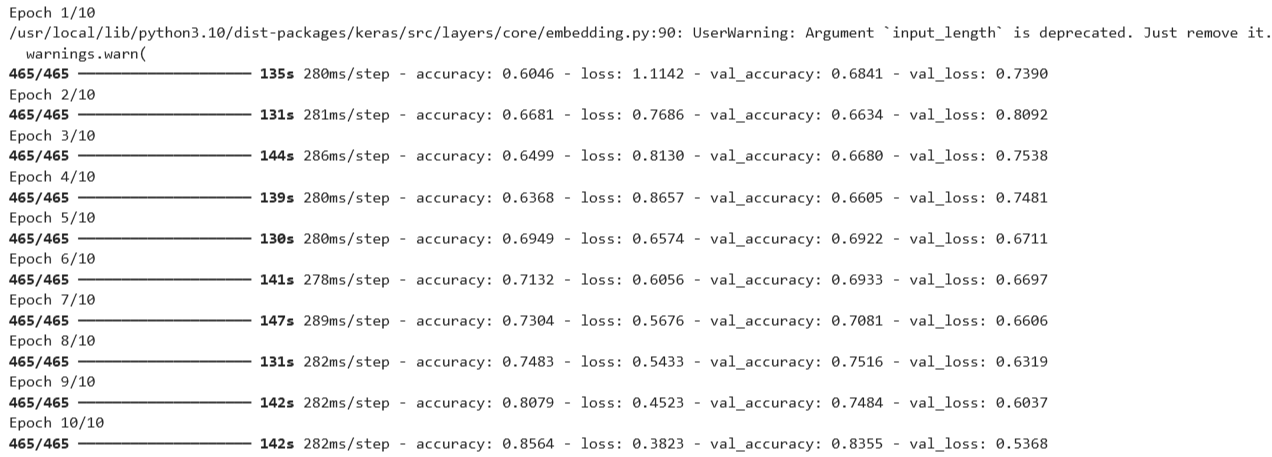
\includegraphics[width=1.0\textwidth]{Images/LSTM Epoch.png}  
    \caption{Output for LSTM Epochs}
    \label{LSTm Epochs}  % Label for referencing the figure
\end{figure}

\begin{figure}[h!]  
    \centering
    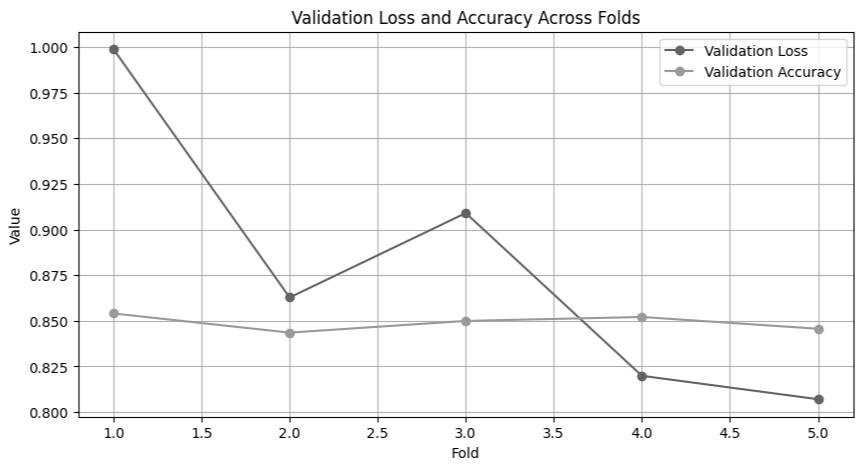
\includegraphics[width=0.9\textwidth]{Images/LSTM LA.png}  
    \caption{LSTM Validation loss and accuracy}
    \label{Accuracy Loss}  % Label for referencing the figure
\end{figure}

\begin{figure}[h!]  
    \centering
    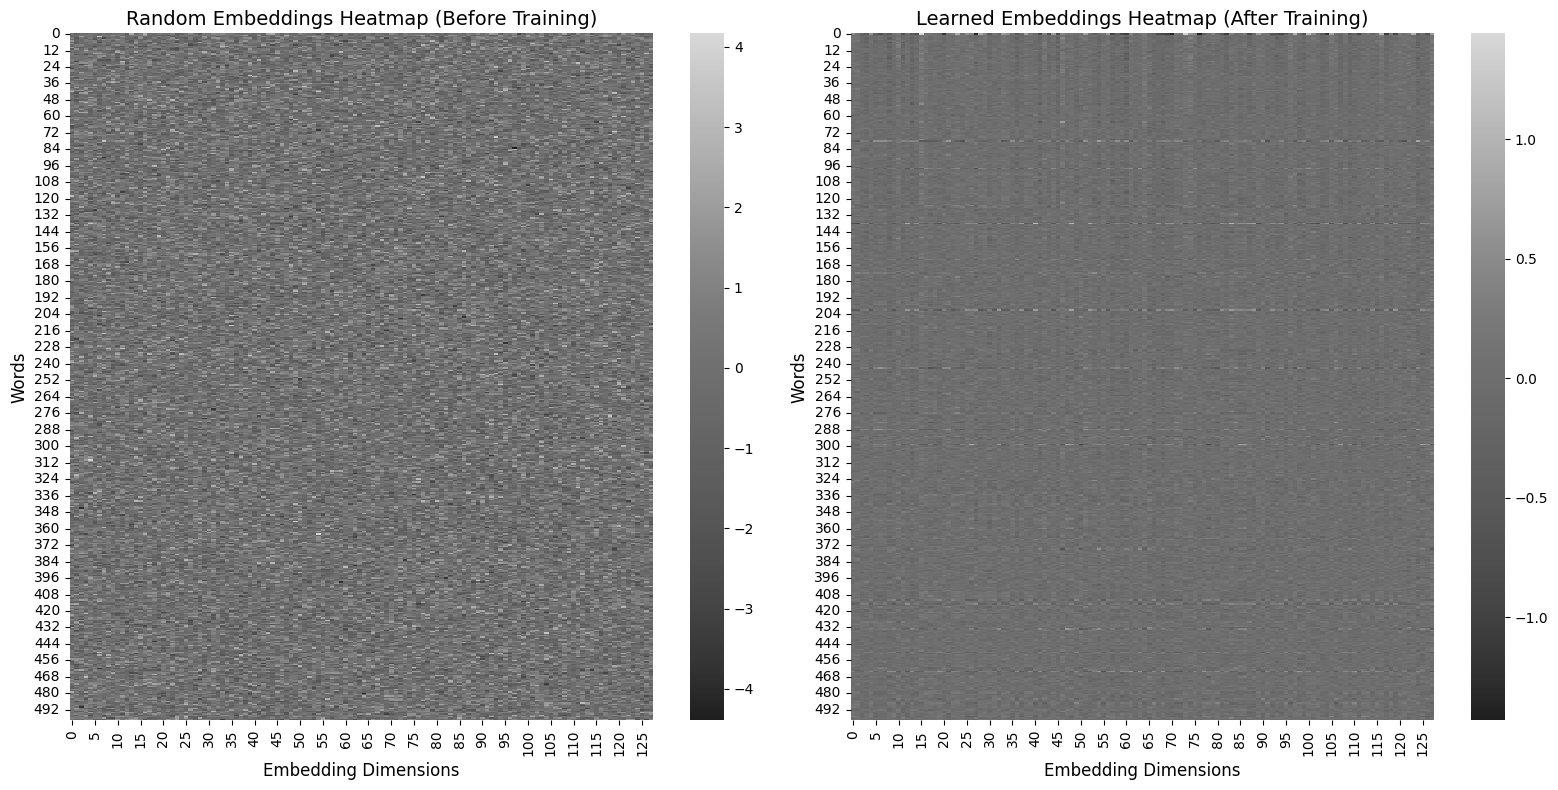
\includegraphics[width=0.85\textwidth]{Images/LSTM EMBED.png}  
    \caption{LSTM Random and Learned Embeddings}
    \label{lstm embed}  % Label for referencing the figure
\end{figure}

\begin{figure}[h!]  
    \centering
    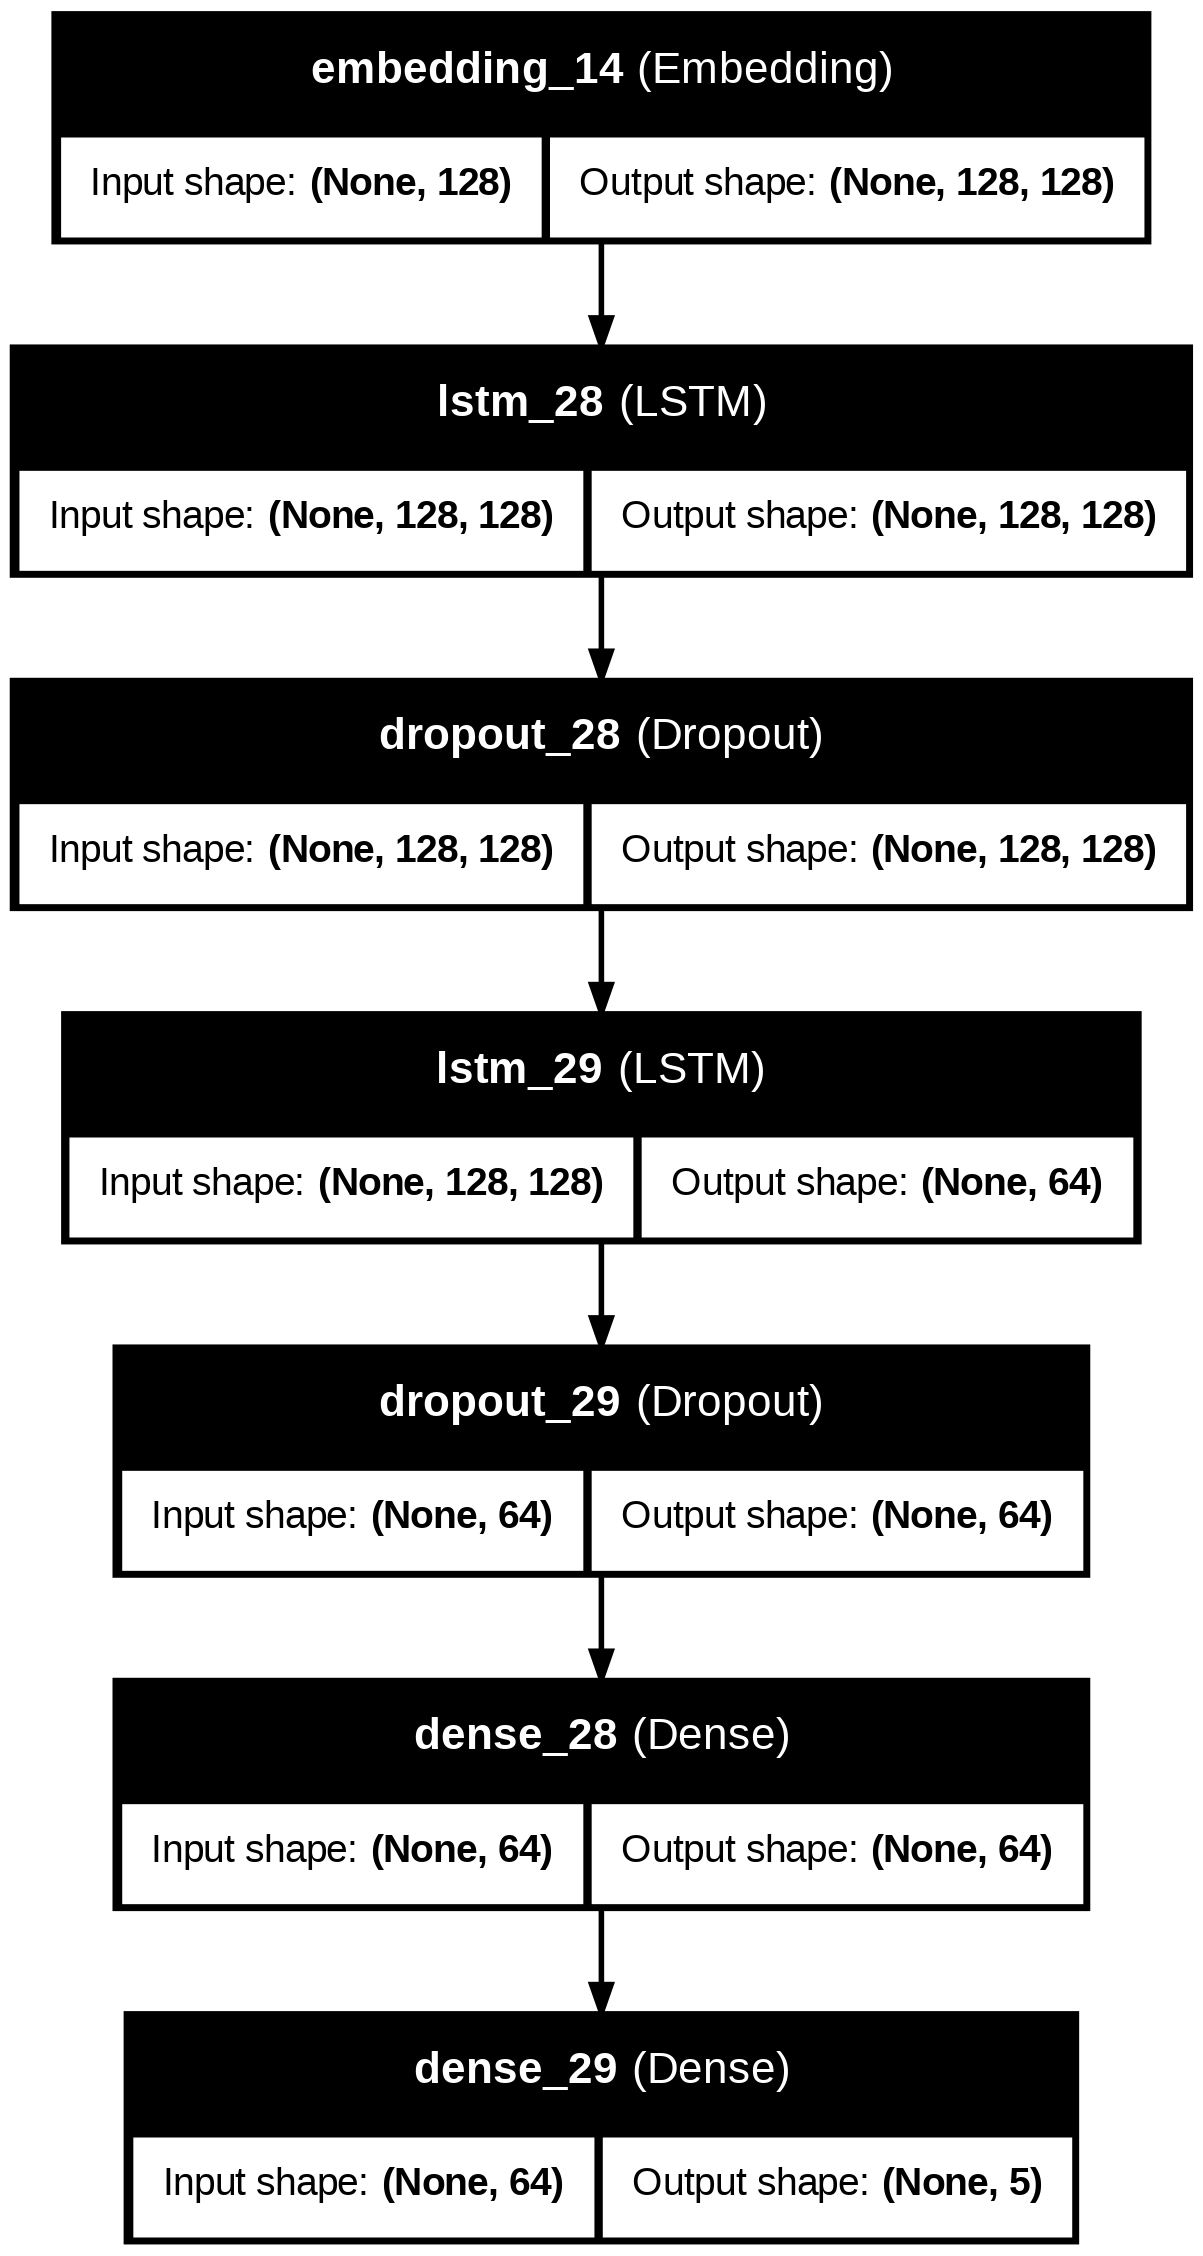
\includegraphics[width=0.45\textwidth]{Images/LSTM MODEL.png}  
    \caption{LSTM Model Architecture}
    \label{lstm arch}  % Label for referencing the figure
\end{figure}

% ---------- hyperparameter tuning

\subsubsection{Hyperparamter Tuning Using RandomizedSearchCV}

\begin{tcolorbox}[colback=gray!5!white, colframe=gray!80!black, boxrule=0.5pt, title=Logistic Regression]
\begin{lstlisting}[language=Python]
import pandas as pd
from sklearn.model_selection import train_test_split, RandomizedSearchCV
from sklearn.feature_extraction.text import CountVectorizer
from sklearn.linear_model import LogisticRegression
from sklearn.metrics import accuracy_score, classification_report

# Load the preprocessed dataset
dataset = pd.read_csv('preprocessed_mental_health.csv')
if 'cleaned_text' not in dataset.columns or 'mental_health_issue' not in dataset.columns:
    raise ValueError("The dataset must have 'cleaned_text' and 'mental_health_issue' columns.")
# Remove rows with missing values in 'cleaned_text' column
dataset.dropna(subset=['cleaned_text'], inplace=True)

# Initialize the CountVectorizer and fit/transform the cleaned text
HPLRvectorizer = CountVectorizer()
X = HPLRvectorizer.fit_transform(dataset['cleaned_text'])

# Prepare the target variable
y = dataset['mental_health_issue']
# Split the dataset into Training and Test Sets
X_train, X_test, y_train, y_test = train_test_split(X, y, test_size=0.2, random_state=42)

# Initialize the Logistic Regression model
HPLRmodel = LogisticRegression(max_iter=200)
# Define the hyperparameter grid for Randomized Search
param_distributions = {
    'C': [0.001, 0.01, 0.1, 1, 10, 100], 'penalty': ['l1', 'l2', 'elasticnet', 'none'], 'solver': ['liblinear', 'saga']}

# Initialize RandomizedSearchCV
random_search = RandomizedSearchCV(estimator=HPLRmodel, param_distributions=param_distributions, n_iter=10, scoring='accuracy', cv=5, n_jobs=-1, random_state=42)

random_search.fit(X_train, y_train)
print("Best Hyperparameters:", random_search.best_params_)
best_modelLR = random_search.best_estimator_
y_pred = best_modelLR.predict(X_test)
\end{lstlisting}
\end{tcolorbox}

\begin{tcolorbox}[colback=gray!5!white, colframe=gray!80!black, boxrule=0.5pt, title=Logistic Regression]
    \begin{lstlisting}[language=Python]
# Evaluate the model
accuracy = accuracy_score(y_test, y_pred)
print(f'Accuracy: {accuracy * 100:.2f}%')

# Print classification report
print("Classification Report:\n", classification_report(y_test, y_pred))
\end{lstlisting}
\end{tcolorbox}

\noindent
The above code demonstrates a machine learning workflow for classifying mental health issues using \texttt{LogisticRegression} with hyperparameter tuning. The dataset is loaded using \texttt{pandas}, and a check ensures the presence of \texttt{'cleaned\_text'} and \texttt{'mental\_health\_issue'} columns. Missing values in \texttt{'cleaned\_text'} are dropped to prevent processing errors. The textual data is transformed into a numerical format using \texttt{CountVectorizer}, which converts text into a bag-of-words representation. The dataset is then split into training and testing sets using \texttt{train\_test\_split}. A logistic regression model is initialized, and the hyperparameter grid is defined, including parameters like \texttt{C} (inverse of regularization strength), \texttt{penalty}, and \texttt{solver}. Hyperparameter tuning is performed using \texttt{RandomizedSearchCV}, which searches for the best model configuration by sampling parameter combinations. The best model is used to make predictions on the test set, and evaluation metrics such as accuracy and a classification report are printed.

\begin{tcolorbox}[colback=gray!5!white, colframe=gray!80!black, boxrule=0.5pt, title=K Nearest Neighbours]
    \begin{lstlisting}[language=Python]
import pandas as pd
from sklearn.model_selection import train_test_split, RandomizedSearchCV
from sklearn.feature_extraction.text import CountVectorizer
from sklearn.neighbors import KNeighborsClassifier
from sklearn.metrics import accuracy_score, classification_report, confusion_matrix

# Load the preprocessed dataset
dataset = pd.read_csv('preprocessed_mental_health.csv')
# Check if 'cleaned_text' and 'mental_health_issue' columns exist
if 'cleaned_text' not in dataset.columns or 'mental_health_issue' not in dataset.columns:
    raise ValueError("The dataset must have 'cleaned_text' and 'mental_health_issue' columns.")
\end{lstlisting}
\end{tcolorbox}

\begin{tcolorbox}[colback=gray!5!white, colframe=gray!80!black, boxrule=0.5pt, title=K Nearest Neighbours]
    \begin{lstlisting}[language=Python]
# Remove rows with missing values in 'cleaned_text' column
dataset.dropna(subset=['cleaned_text'], inplace=True)

# Initialize the CountVectorizer and fit/transform the cleaned text
HPTKNNvectorizer = CountVectorizer()
X = HPTKNNvectorizer.fit_transform(dataset['cleaned_text'])

# Prepare the target variable
y = dataset['mental_health_issue']

# Split the dataset into Training and Test Sets
X_train, X_test, y_train, y_test = train_test_split(X, y, test_size=0.2, random_state=42)

# Initialize the k-NN classifier
knn = KNeighborsClassifier()

# Define the hyperparameter grid for Randomized Search
param_distributions = {
    'n_neighbors': [3, 4, 5, 6, 7, 8, 9, 10, 11, 12, 13, 15, 14, 15, 16, 17, 18, 19, 20],
        # Different values for number of neighbors
    'metric': ['euclidean', 'manhattan', 'chebyshev', 'minkowski'],  # Different distance metrics
    'weights': ['uniform', 'distance']  # Weighing options for neighbors
}

# Initialize RandomizedSearchCV
random_search = RandomizedSearchCV(estimator=knn, param_distributions=param_distributions,
                                    n_iter=10, scoring='accuracy', cv=5, n_jobs=-1, random_state=42)

# Fit RandomizedSearchCV
random_search.fit(X_train, y_train)

# Best hyperparameters from Random Search
print("Best Hyperparameters:", random_search.best_params_)

# Best model from Random Search
best_knn = random_search.best_estimator_

# Make predictions using the best model
y_pred = best_knn.predict(X_test)
\end{lstlisting}
\end{tcolorbox}

\begin{tcolorbox}[colback=gray!5!white, colframe=gray!80!black, boxrule=0.5pt, title=K Nearest Neighbours]
    \begin{lstlisting}[language=Python]
# Evaluate the model
accuracy = accuracy_score(y_test, y_pred)
print(f'Accuracy: {accuracy * 100:.2f}%')

# Print classification report
print("Classification Report:\n", classification_report(y_test, y_pred))

# Print confusion matrix
print("Confusion Matrix:\n", confusion_matrix(y_test, y_pred))
    \end{lstlisting}
\end{tcolorbox}

\noindent
This code implements a k-Nearest Neighbors (k-NN) classifier for classifying mental health issues from text data using hyperparameter tuning via RandomizedSearchCV. First, it loads a preprocessed dataset, ensuring the existence of critical columns, \texttt{cleaned\_text} (features) and \texttt{mental\_health\_issue} (target). Rows with missing values in the \texttt{cleaned\_text} column are removed to maintain data integrity. The text is vectorized into numerical format using \texttt{CountVectorizer}, converting text into a bag-of-words model. The features (\(X\)) and target (\(y\)) are split into training (80\%) and test (20\%) datasets to ensure proper model evaluation. The k-NN model is initialized without predefined parameters, and a hyperparameter grid is defined for tuning. This grid explores various values for the number of neighbors (\texttt{n\_neighbors}), distance metrics (\texttt{metric}), and neighbor weighting options (\texttt{weights}). \texttt{RandomizedSearchCV} is then used to optimize these parameters by training multiple k-NN models with combinations from the grid, evaluating them with 5-fold cross-validation, and scoring based on accuracy. The best combination of hyperparameters is identified and used to configure the final k-NN model. The model is then tested on unseen data (test set), and its performance is evaluated by calculating the accuracy, a classification report detailing precision, recall, F1-score for each class, and a confusion matrix showing true vs. predicted classifications. This approach balances computational efficiency with robustness, enabling the selection of an optimized k-NN model for mental health classification.


\begin{tcolorbox}[colback=gray!5!white, colframe=gray!80!black, boxrule=0.5pt, title=Support Vector Machine]
    \begin{lstlisting}[language=Python]
import pandas as pd
from sklearn.model_selection import train_test_split, RandomizedSearchCV
from sklearn.feature_extraction.text import CountVectorizer
from sklearn.svm import SVC
from sklearn.metrics import accuracy_score, classification_report
\end{lstlisting}
\end{tcolorbox}

\begin{tcolorbox}[colback=gray!5!white, colframe=gray!80!black, boxrule=0.5pt, title=Support Vector Machine]
    \begin{lstlisting}[language=Python]
# Load the preprocessed dataset
dataset = pd.read_csv('preprocessed_mental_health.csv')

# Check if 'cleaned_text' and 'mental_health_issue' columns exist
if 'cleaned_text' not in dataset.columns or 'mental_health_issue' not in dataset.columns:
    raise ValueError("The dataset must have 'cleaned_text' and 'mental_health_issue' columns.")

# Remove rows with missing values in 'cleaned_text' column
dataset.dropna(subset=['cleaned_text'], inplace=True)

# Initialize the CountVectorizer and fit/transform the cleaned text
vectorizer = CountVectorizer()
X = vectorizer.fit_transform(dataset['cleaned_text'])

# Prepare the target variable
y = dataset['mental_health_issue']

# Split the dataset into Training and Test Sets
X_train, X_test, y_train, y_test = train_test_split(X, y, test_size=0.2, random_state=42)

# Initialize the SVC model
model = SVC()

# Define the hyperparameter grid for Randomized Search
param_distributions = {
    'C': [0.1, 1, 10, 100],               # Regularization parameter
    'kernel': ['linear', 'rbf', 'poly'],  # Kernel types
    'gamma': ['scale', 'auto', 0.1, 1],   # Kernel coefficient for 'rbf', 'poly', and 'sigmoid'
}

# Initialize RandomizedSearchCV
random_search = RandomizedSearchCV(estimator=model, param_distributions=param_distributions,
                                    n_iter=10, scoring='accuracy', cv=5, n_jobs=-1, random_state=42)

# Fit RandomizedSearchCV
random_search.fit(X_train, y_train)
\end{lstlisting}
\end{tcolorbox}

\begin{tcolorbox}[colback=gray!5!white, colframe=gray!80!black, boxrule=0.5pt, title=Support Vector Machine]
    \begin{lstlisting}[language=Python]
# Best hyperparameters from Random Search
print("Best Hyperparameters:", random_search.best_params_)

# Best model from Random Search
best_model = random_search.best_estimator_

# Make predictions using the best model
y_pred = best_model.predict(X_test)

# Evaluate the model
accuracy = accuracy_score(y_test, y_pred)
print(f'Accuracy: {accuracy * 100:.2f}%')

# Print classification report
print("Classification Report:\n", classification_report(y_test, y_pred))
\end{lstlisting}
\end{tcolorbox}

\noindent
This code implements a Support Vector Classifier (SVC) for classifying mental health issues from text data using hyperparameter tuning via RandomizedSearchCV. It begins by loading a preprocessed dataset and ensuring that essential columns, \texttt{cleaned\_text} (features) and \texttt{mental\_health\_issue} (target), are present. Any rows with missing values in the \texttt{cleaned\_text} column are removed to ensure clean data. The text is then vectorized into a numerical format using \texttt{CountVectorizer}, transforming it into a bag-of-words representation. The features (\(X\)) and target (\(y\)) are split into training (80\%) and test (20\%) sets for model validation. The SVC model is initialized without predefined hyperparameters, and a hyperparameter grid is defined for tuning. This grid includes different values for the regularization parameter (\texttt{C}), kernel types (\texttt{kernel}), and the kernel coefficient (\texttt{gamma}). \texttt{RandomizedSearchCV} is employed to find the best combination of these parameters by evaluating multiple models with various hyperparameter combinations through 5-fold cross-validation, using accuracy as the scoring metric. The best set of hyperparameters is selected to configure the final SVC model. The model is then evaluated on the test set by making predictions, and its performance is measured by calculating the accuracy, as well as generating a classification report that includes precision, recall, and F1-score for each class. This approach ensures the selection of the most optimized SVC model for the classification of mental health issues from text data.

\begin{tcolorbox}[colback=gray!5!white, colframe=gray!80!black, boxrule=0.5pt, title=Naive Bayes]
    \begin{lstlisting}[language=Python]
import pandas as pd
from sklearn.model_selection import train_test_split, RandomizedSearchCV
from sklearn.feature_extraction.text import CountVectorizer
from sklearn.naive_bayes import MultinomialNB
from sklearn.metrics import accuracy_score, classification_report, confusion_matrix
from scipy.stats import uniform

# Load the preprocessed dataset
dataset = pd.read_csv('preprocessed_mental_health.csv')

# Check if 'cleaned_text' and 'mental_health_issue' columns exist
if 'cleaned_text' not in dataset.columns or 'mental_health_issue' not in dataset.columns:
    raise ValueError("The dataset must have 'cleaned_text' and 'mental_health_issue' columns.")

# Remove rows with missing values in 'cleaned_text' column
dataset.dropna(subset=['cleaned_text'], inplace=True)

# Initialize the CountVectorizer and fit/transform the cleaned text
vectorizer = CountVectorizer()
X = vectorizer.fit_transform(dataset['cleaned_text'])

# Prepare the target variable
y = dataset['mental_health_issue']

# Split the dataset into Training and Test Sets
X_train, X_test, y_train, y_test = train_test_split(X, y, test_size=0.2, random_state=42)

# Initialize the Naive Bayes model
naive_bayes_model = MultinomialNB()

# Define the parameter distribution for Randomized Search
param_distributions = {
    'alpha': uniform(0.001, 5.0)  # Sampling alpha from a uniform distribution
}
\end{lstlisting}
\end{tcolorbox}

\begin{tcolorbox}[colback=gray!5!white, colframe=gray!80!black, boxrule=0.5pt, title=Naive Bayes]
    \begin{lstlisting}[language=Python]
# Initialize RandomizedSearchCV
random_search = RandomizedSearchCV(estimator=naive_bayes_model, param_distributions=param_distributions,
                                    n_iter=10, scoring='accuracy', cv=5, n_jobs=-1, random_state=42)

# Fit RandomizedSearchCV
random_search.fit(X_train, y_train)

# Best hyperparameters from Random Search
print("Best Hyperparameters:", random_search.best_params_)

# Best model from Random Search
best_model = random_search.best_estimator_

# Make predictions using the best model
y_pred = best_model.predict(X_test)

# Evaluate the model
accuracy = accuracy_score(y_test, y_pred)
print(f'Accuracy: {accuracy * 100:.2f}%')

# Print classification report
print("Classification Report:\n", classification_report(y_test, y_pred))

# Print confusion matrix
print("Confusion Matrix:\n", confusion_matrix(y_test, y_pred))        
    \end{lstlisting}
\end{tcolorbox}

\noindent
This code implements a Naive Bayes classifier using the MultinomialNB algorithm to classify mental health issues from text data, with hyperparameter tuning via RandomizedSearchCV. The dataset is first loaded, ensuring the required columns, \texttt{cleaned\_text} (features) and \texttt{mental\_health\_issue} (target), exist. Rows with missing values in the \texttt{cleaned\_text} column are removed to maintain data quality. The text is vectorized using \texttt{CountVectorizer}, converting it into a bag-of-words representation. The features (\(X\)) and target (\(y\)) are then split into training (80\%) and test (20\%) sets to facilitate proper evaluation. The Naive Bayes model is initialized, and a parameter distribution for \texttt{alpha} is defined using a uniform distribution, sampling values between 0.001 and 5.0. \texttt{RandomizedSearchCV} is utilized to explore different values for \texttt{alpha} over 10 iterations, using 5-fold cross-validation and accuracy as the scoring metric. The best hyperparameters are identified and used to configure the final Naive Bayes model. The model is then tested on the unseen data (test set).

% ---------- transformer -------
\subsubsection{Tranformer based model for classification}

\begin{tcolorbox}[colback=gray!5!white, colframe=gray!80!black, boxrule=0.5pt, title=Importing Libraries]
    \begin{lstlisting}[language=Python]
import numpy as np
import pandas as pd
from sklearn.preprocessing import LabelEncoder
from sklearn.metrics import confusion_matrix, ConfusionMatrixDisplay
from tensorflow.keras.layers import MultiHeadAttention, Input, Dense, Embedding, GlobalAveragePooling1D, LayerNormalization, Layer
from tensorflow.keras.models import Model, Sequential
from tensorflow.keras.utils import to_categorical
from tensorflow.keras.layers import TextVectorization
import matplotlib.pyplot as plt
from tensorflow.data import Dataset
from tensorflow import convert_to_tensor, string, float32, shape, range, reshape
    \end{lstlisting}
\end{tcolorbox}

\noindent
The provided Python code imports a set of essential libraries and modules used for data processing, machine learning, and neural network construction. NumPy and pandas are used for numerical computations and data manipulation, while scikit-learn provides tools like label encoding and confusion matrix evaluation. TensorFlow modules enable the construction of advanced deep learning architectures with layers such as multi-head attention and embeddings, alongside utilities for text vectorization and categorical encoding. Matplotlib is utilized for visualizations, and TensorFlow's Dataset API facilitates efficient data handling and pipeline creation for training models.

\begin{tcolorbox}[colback=gray!5!white, colframe=gray!80!black, boxrule=0.5pt, title=Load Dataset]
    \begin{lstlisting}[language=Python]
from google.colab import files

# Upload the file
uploaded = files.upload()
# Load dataset
file_path = 'preprocessed_mental_health.csv'
data = pd.read_csv(file_path)

# Drop rows with missing cleaned_text
data = data.dropna(subset=['cleaned_text'])
# Extract features and labels
texts = data['cleaned_text'].astype(str).values
labels = data['mental_health_issue'].astype(str).values
    \end{lstlisting}
\end{tcolorbox}

\noindent
This code snippet uses Google Colab's `files` module to upload datasets interactively, enabling easy integration with cloud-based environments. It then loads a dataset in CSV format using pandas and preprocesses the data by dropping rows with missing values in the `cleaned\_text` column. The `cleaned\_text` column is used to extract the textual features, and the `mental\_health\_issue` column provides the corresponding labels for classification tasks, both stored as NumPy arrays.

\begin{tcolorbox}[colback=gray!5!white, colframe=gray!80!black, boxrule=0.5pt, title=Processing Labels and Text Vectorization]
    \begin{lstlisting}[language=Python]
# Encode the labels
label_encoder = LabelEncoder()
encoded_labels = label_encoder.fit_transform(labels)
categorical_labels = to_categorical(encoded_labels)

# Get class names
class_names = label_encoder.classes_
print("Classes:", class_names)
# Define parameters
vocab_size = 25000
sequence_length = 300

# Vectorization layer
vectorize_layer = TextVectorization(max_tokens=vocab_size, output_sequence_length=sequence_length)

# Adapt vectorizer to texts
vectorize_layer.adapt(Dataset.from_tensor_slices(texts))
# Vectorize text data
texts_vectorized = vectorize_layer(convert_to_tensor(texts, dtype=string))
    \end{lstlisting}
\end{tcolorbox}

This code snippet encodes textual labels into numerical format using the `LabelEncoder` from scikit-learn and transforms them into categorical labels suitable for deep learning models. The class names are retrieved and displayed for reference. A `TextVectorization` layer is defined with specified vocabulary size and sequence length to preprocess text data into numerical format. The vectorization layer is adapted to the text dataset, and the texts are vectorized into fixed-length sequences for model input.

\begin{tcolorbox}[colback=gray!5!white, colframe=gray!80!black, boxrule=0.5pt, title=Define Transformer Model]
    \begin{lstlisting}[language=Python]
class EmbeddingLayer(Layer):
    def __init__(self, sequence_length, vocab_size, embed_dim):
        super(EmbeddingLayer, self).__init__()
        self.word_embedding = Embedding(input_dim=vocab_size, output_dim=embed_dim)
        self.position_embedding = Embedding(input_dim=sequence_length, output_dim=embed_dim)

    def call(self, tokens):
        sequence_length = shape(tokens)[-1]
        positions = range(start=0, limit=sequence_length, delta=1)
        positions_encoding = self.position_embedding(positions)
        words_encoding = self.word_embedding(tokens)
        return positions_encoding + words_encoding

class EncoderLayer(Layer):
    def __init__(self, total_heads, total_dense_units, embed_dim):
        super(EncoderLayer, self).__init__()
        self.multihead = MultiHeadAttention(num_heads=total_heads, key_dim=embed_dim)
        self.nnw = Sequential([Dense(total_dense_units, activation="relu"), Dense(embed_dim)])
        self.normalize_layer = LayerNormalization()

    def call(self, inputs):
        attn_output = self.multihead(inputs, inputs)
        normalize_attn = self.normalize_layer(inputs + attn_output)
        nnw_output = self.nnw(normalize_attn)
        final_output = self.normalize_layer(normalize_attn + nnw_output)
        return final_output

# Model parameters
embed_dim = 64
num_heads = 2
total_dense_units = 60

# Define the model
inputs = Input(shape=(sequence_length,))
embedding_layer = EmbeddingLayer(sequence_length, vocab_size, embed_dim)
encoder_layer = EncoderLayer(num_heads, total_dense_units, embed_dim)
\end{lstlisting}
\end{tcolorbox}
\begin{tcolorbox}[colback=gray!5!white, colframe=gray!80!black, boxrule=0.5pt, title=Define Transformer Model]
    \begin{lstlisting}[language=Python]
emb = embedding_layer(inputs)
enc = encoder_layer(emb)
pool = GlobalAveragePooling1D()(enc)
dense = Dense(total_dense_units, activation="relu")(pool)
outputs = Dense(len(class_names), activation="softmax")(dense)

transformer_model = Model(inputs=inputs, outputs=outputs)
transformer_model.compile(optimizer="adamw", loss="categorical_crossentropy", metrics=['accuracy'])
transformer_model.summary()
    \end{lstlisting}
\end{tcolorbox}

\noindent
This code snippet defines a transformer-based model for text classification. The `EmbeddingLayer` class creates embeddings for both words and their positions in the sequence, allowing the model to consider positional context. The `EncoderLayer` class implements an attention mechanism using multi-head attention and dense layers, followed by normalization for improved training stability. The model incorporates these layers to process tokenized input sequences, aggregates information with global pooling, and predicts class probabilities through dense layers with softmax activation. The model is compiled with the AdamW optimizer and categorical crossentropy loss for multi-class classification tasks.

\begin{figure}[h!]  
    \centering
    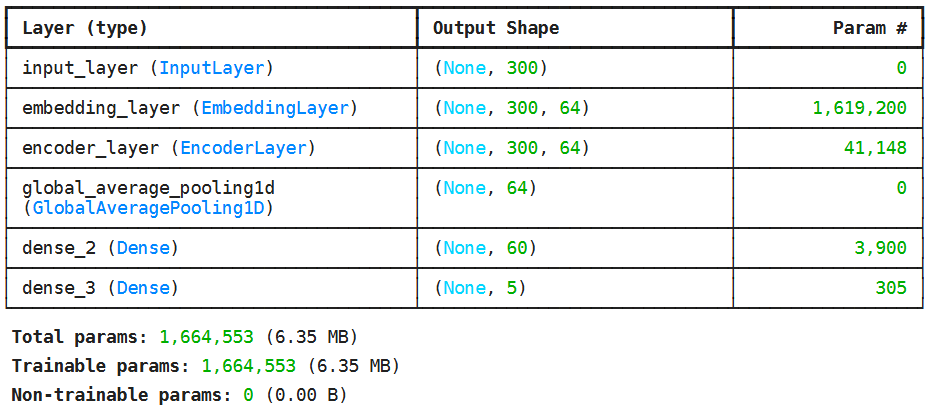
\includegraphics[width=1.0\textwidth]{Images/TMODEL SUM.png}  
    \caption{Transformer Model Summary}
    \label{trans sum}  % Label for referencing the figure
\end{figure}

\begin{tcolorbox}[colback=gray!5!white, colframe=gray!80!black, boxrule=0.5pt, title=Train Transformer Model]
    \begin{lstlisting}[language=Python]
# Split data into train and validation
from sklearn.model_selection import train_test_split
import numpy as np # Import numpy

# Convert the TensorFlow tensor to a NumPy array
texts_vectorized_np = texts_vectorized.numpy()

# Now perform the split
X_train, X_val, y_train, y_val = train_test_split(
    texts_vectorized_np, categorical_labels, test_size=0.2, random_state=42
)

# Train the model
history = transformer_model.fit(
    X_train, y_train,
    validation_data=(X_val, y_val),
    batch_size=32,
    epochs=5
)
    \end{lstlisting}
\end{tcolorbox}

\noindent
This code performs the crucial steps of splitting the dataset into training and validation sets, followed by training the transformer-based model. The \texttt{train\_test\_split} function from the \texttt{sklearn.model\_selection} module is used to divide the data, ensuring that 20\% of the data is set aside for validation while maintaining a random state for reproducibility. Before splitting, the vectorized text data, originally in TensorFlow tensor format, is converted to a NumPy array using the \texttt{numpy()} method. This conversion facilitates seamless integration with scikit-learn functions. The training process involves the \texttt{fit} method of the transformer model. Here, the training features (\texttt{X\_train}) and labels (\texttt{y\_train}) are passed to the model, alongside the validation data (\texttt{X\_val} and \texttt{y\_val}) for evaluating the model's performance on unseen data during training. A batch size of 32 ensures that the data is processed in manageable chunks, balancing computational efficiency and learning stability. The training is conducted over 5 epochs, allowing the model to iteratively adjust its weights to minimize the loss function. The resulting \texttt{history} object captures the training and validation metrics for each epoch, which can be used for performance analysis and visualization.

\pagebreak

\begin{figure}[h!]  
    \centering
    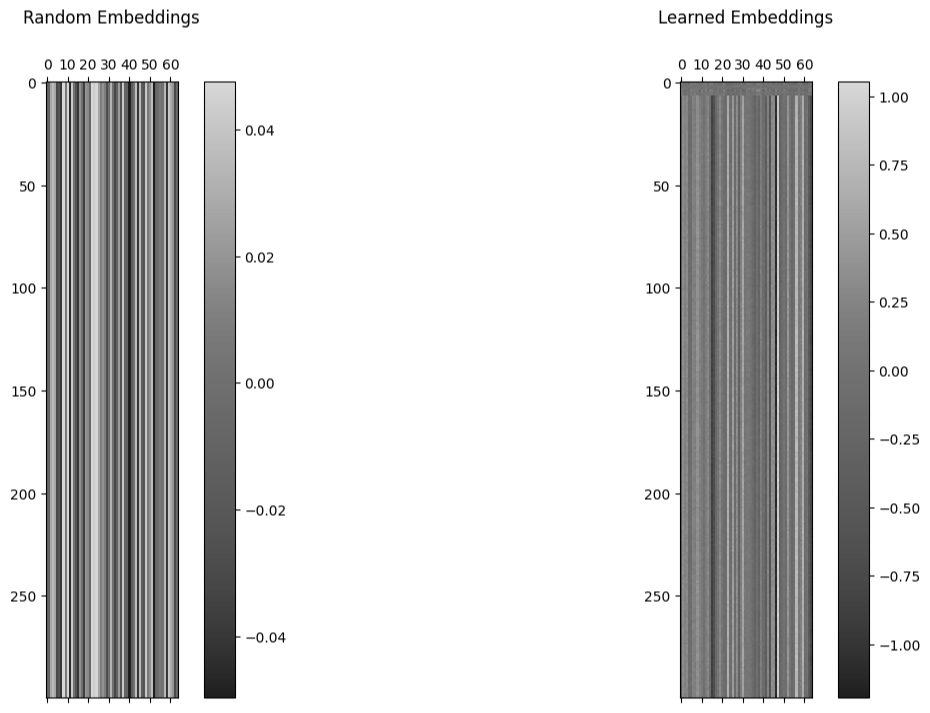
\includegraphics[width=1.0\textwidth]{Images/T EMBED.png}  
    \caption{Transformer Model Random and Learned Embeddings}
    \label{lstm t embed}  % Label for referencing the figure
\end{figure}

\begin{figure}[h!]  
    \centering
    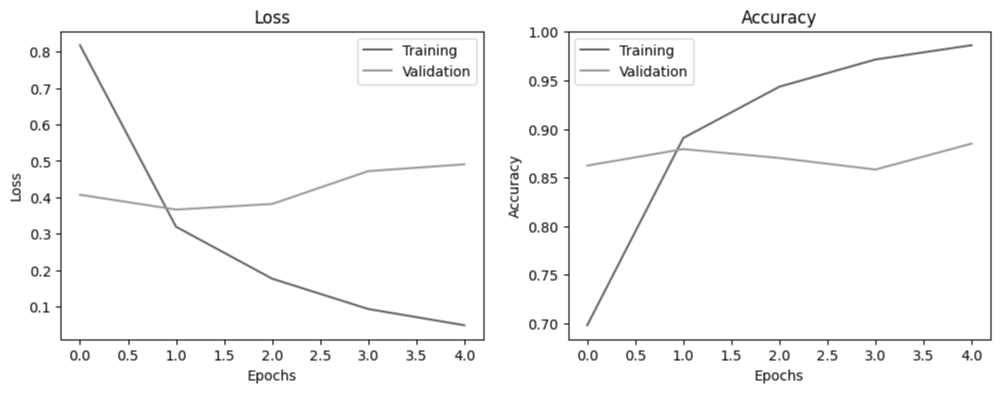
\includegraphics[width=1.0\textwidth]{Images/T LOSS EPOCH.png}  
    \caption{Transformer Epoch, Loss, Accuracy}
    \label{lstm t epch}  % Label for referencing the figure
\end{figure}

\pagebreak

% --------- ENSEMBLE LEARNING 1----------
\subsubsection{Ensemble Model 1 (Stacking with Meta-Learner : Logistic Regression)}
\noindent
\textbf{Base Model : Logistic Regression, XGBoost. }

\begin{tcolorbox}[colback=gray!5!white, colframe=gray!80!black, boxrule=0.5pt, title=Ensemble Model 1 : Loading and Preprocessing]
    \begin{lstlisting}[language=Python]
import pickle
from sklearn.ensemble import StackingClassifier
from sklearn.linear_model import LogisticRegression
from sklearn.metrics import accuracy_score, classification_report
import xgboost as xgb
import pandas as pd

# Load the Logistic Regression model and vectorizer
with open('LRmodel.pkl', 'rb') as file:
    lr_model = pickle.load(file)
with open('LRvectorizer.pkl', 'rb') as file:
    lr_vectorizer = pickle.load(file)
# Load the XGBoost model, label encoder, and TF-IDF vectorizer
with open('xgb_model.pkl', 'rb') as file:
    xgb_model = pickle.load(file)
with open('label_encoder.pkl', 'rb') as file:
    label_encoder = pickle.load(file)
with open('tfidf_vectorizer.pkl', 'rb') as file:
    tfidf_vectorizer = pickle.load(file)
    \end{lstlisting}
\end{tcolorbox}

\noindent
This Python code is centered around preparing a machine learning workflow by loading pre-trained models and their corresponding preprocessing tools. It begins by importing essential libraries for model evaluation and stacking. The \texttt{pickle} library is specifically used to load serialized Python objects, enabling the restoration of previously trained models and utilities saved as \texttt{.pkl} files. The first part of the code loads a Logistic Regression model along with its associated vectorizer. The Logistic Regression model is deserialized from the \texttt{LRmodel.pkl} file, which represents a trained model capable of predicting outcomes based on vectorized text data. The corresponding vectorizer, stored in \texttt{LRvectorizer.pkl}, is also loaded. This vectorizer, likely a \texttt{CountVectorizer}, converts raw text into numerical feature vectors, which serve as the input for the Logistic Regression model. By loading these components, the workflow ensures consistency with the preprocessing and modeling steps used during training. In the next section, the code loads an XGBoost model alongside its associated tools. The XGBoost model is deserialized from \texttt{xgb\_model.pkl} and represents another trained model designed to classify text data. To facilitate this, the code also loads a label encoder from \texttt{label\_encoder.pkl}. The label encoder is responsible for mapping textual class labels (e.g., "depression" or "normal") to numerical values required by machine learning models. Furthermore, the \texttt{tfidf\_vectorizer.pkl} is loaded to preprocess text data using the Term Frequency-Inverse Document Frequency (TF-IDF) approach, which captures the importance of words in a document relative to a corpus. This ensures that the input text is transformed in a manner consistent with the original training setup of the XGBoost model. The design of this code emphasizes efficiency and consistency by leveraging pre-trained components. Instead of retraining models, it restores them from their serialized forms, enabling immediate use for predictions or integration into ensemble learning setups. This approach also ensures that text preprocessing remains identical to the training phase, avoiding discrepancies in input data handling. By combining these tools, the foundation is laid for complex tasks such as making predictions or building advanced models like stacked classifiers.

\begin{tcolorbox}[colback=gray!5!white, colframe=gray!80!black, boxrule=0.5pt, title=Ensemble Model 1 : Data Preparation]
\begin{lstlisting}[language=Python]
# Load the test dataset
data = pd.read_csv('preprocessed_mental_health.csv')

# Check if 'cleaned_text' column exists
if 'cleaned_text' not in data.columns:
    raise ValueError("The dataset must have a 'cleaned_text' column.")

# Remove rows with missing values in 'cleaned_text'
data.dropna(subset=['cleaned_text'], inplace=True)

# Split features and target
X_test = data['cleaned_text']
y_test = data['mental_health_issue']

# Encode target labels
y_test = label_encoder.transform(y_test)

# Transform the text using the respective vectorizers
X_test_lr = lr_vectorizer.transform(X_test)  # Logistic Regression vectorizer
X_test_xgb = tfidf_vectorizer.transform(X_test)  # XGBoost vectorizer
\end{lstlisting}
\end{tcolorbox}
    
\noindent
This code snippet focuses on preparing the test dataset for evaluation with pre-trained machine learning models, specifically Logistic Regression and XGBoost. First, the test dataset is loaded from a CSV file named \texttt{preprocessed\_mental\_health.csv} using \texttt{pd.read\_csv}. The dataset is expected to have been preprocessed earlier, containing features and corresponding labels. The code then checks for the existence of a critical column named \texttt{cleaned\_text}. If this column is missing, a \texttt{ValueError} is raised, ensuring that the dataset meets the required format for subsequent steps. Next, the code removes rows with missing values in the \texttt{cleaned\_text} column using \texttt{data.dropna}. This step ensures the dataset is clean and free of incomplete rows that could potentially cause errors during text transformation or model evaluation. After this cleaning process, the dataset is split into features (\texttt{X\_test}) and target labels (\texttt{y\_test}). The features contain the preprocessed text, while the target labels represent the mental health issues corresponding to each text entry. The target labels in \texttt{y\_test} are then encoded into numerical format using a preloaded \texttt{label\_encoder}. This encoding is crucial because machine learning models require numerical representations of categorical labels for classification tasks. By transforming the labels to integers, the encoded labels are consistent with the classes used during the model's training phase. Finally, the text data in \texttt{X\_test} is vectorized using two pre-trained vectorizers. The \texttt{lr\_vectorizer}, likely a \texttt{CountVectorizer} or similar, is applied to produce feature vectors suitable for the Logistic Regression model. Simultaneously, the \texttt{tfidf\_vectorizer} is applied to transform the same text data into feature vectors optimized for the XGBoost model. These transformations ensure that the test data aligns with the feature representations learned by the respective models during training. This setup allows for seamless evaluation of the Logistic Regression and XGBoost models on the same dataset, maintaining consistency with their training configurations.

\begin{tcolorbox}[colback=gray!5!white, colframe=gray!80!black, boxrule=0.5pt, title=Ensemble Model 1 : Combine Base Model Predictions]
\begin{lstlisting}[language=Python]
import numpy as np

# Get predictions from the base models
lr_predictions_proba = lr_model.predict_proba(X_test_lr)
xgb_predictions_proba = xgb_model.predict_proba(X_test_xgb)

# Combine predictions as new features
stacked_features = np.hstack((lr_predictions_proba, xgb_predictions_proba))
\end{lstlisting}
\end{tcolorbox}

\noindent
This Python code demonstrates a fundamental step in stacking ensemble learning by combining the prediction probabilities of base models into a single feature set. The process begins with obtaining predictions from two pre-trained models: a Logistic Regression model (\texttt{lr\_model}) and an XGBoost model (\texttt{xgb\_model}). These models generate class probability distributions for the test dataset, which are then used as input features for a meta-learner in an ensemble framework. First, the code uses the \texttt{predict\_proba} method of each model to calculate the probabilities associated with each class for every test instance. For the Logistic Regression model, the feature set (\texttt{X\_test\_lr}) is passed to \texttt{lr\_model.predict\_proba}, producing a 2D array (\texttt{lr\_predictions\_proba}) where each row contains the class probabilities for a corresponding instance. Similarly, the XGBoost model processes its input features (\texttt{X\_test\_xgb}) to generate a comparable 2D array (\texttt{xgb\_predictions\_proba}) of class probabilities. Next, the code combines these probability arrays to form a new feature set, referred to as \texttt{stacked\_features}. This is accomplished using the \texttt{np.hstack} function from the NumPy library, which horizontally stacks the arrays column-wise. The resulting \texttt{stacked\_features} array contains concatenated probability distributions from both models for each instance. For example, if there are three classes and 100 instances, the combined feature set will have 100 rows and six columns (three from each model). This stacked feature set serves as input to a meta-learner, enabling it to make final predictions by leveraging the strengths of both base models. By integrating predictions in this manner, the stacking approach aims to improve classification performance by reducing errors associated with individual models. The meta-learner effectively learns how to optimally combine these predictions to produce more accurate outcomes.
    
\begin{tcolorbox}[colback=gray!5!white, colframe=gray!80!black, boxrule=0.5pt, title=Ensemble Model 1 : Train Meta-Learner]
\begin{lstlisting}[language=Python]
# Train meta-learner using combined features (optional step if not pre-trained)
X_train_meta, y_train_meta = stacked_features, y_test  # Example using test data as meta-training data

meta_learner = LogisticRegression(max_iter=5000)
meta_learner.fit(X_train_meta, y_train_meta)

# Save the trained meta-learner
with open('meta_learner.pkl', 'wb') as file:
    pickle.dump(meta_learner, file)
\end{lstlisting}
\end{tcolorbox}

\noindent
This Python code focuses on training a meta-learner in the context of stacking ensemble learning. A meta-learner is a secondary machine learning model trained on the outputs of base models, with the goal of combining their predictions to achieve higher accuracy and robustness. The first step involves defining the training data for the meta-learner. The variable \texttt{X\_train\_meta} is set to the combined feature set (\texttt{stacked\_features}), which contains the concatenated prediction probabilities from base models like Logistic Regression and XGBoost. These features represent the likelihood of each class for every instance, as estimated by the base models. The variable \texttt{y\_train\_meta} holds the true labels (\texttt{y\_test}), which are used as the target variable for training the meta-learner. The code then initializes a Logistic Regression model as the meta-learner. The parameter \texttt{max\_iter=5000} ensures that the optimization process has sufficient iterations to converge, particularly for complex datasets or large feature sets. The \texttt{fit} method is called to train the meta-learner using the stacked features and corresponding labels. During this training process, the meta-learner learns how to optimally combine the prediction probabilities from the base models to produce more accurate final predictions. After training, the code saves the meta-learner to a file named \texttt{meta\_learner.pkl} using the \texttt{pickle.dump} function. This step serializes the trained model, enabling its reuse for future predictions without needing to retrain it. By saving the meta-learner, the workflow becomes more efficient, as the combined expertise of the base models and the meta-learner can be leveraged in subsequent tasks. This approach exemplifies the flexibility and power of stacking ensemble learning, where a meta-learner synthesizes the strengths of multiple base models to enhance predictive performance. The ability to save the meta-learner ensures that this improved model can be deployed in practical applications with minimal computational overhead.
    

\begin{tcolorbox}[colback=gray!5!white, colframe=gray!80!black, boxrule=0.5pt, title=Ensemble Model 1 : Evaluate Meta-Learner and Ensemble Model]
\begin{lstlisting}[language=Python]
from sklearn.metrics import confusion_matrix

# Load the pre-trained meta-learner
with open('meta_learner.pkl', 'rb') as file:
    meta_learner = pickle.load(file)

# Predict using the meta-learner
final_predictions = meta_learner.predict(stacked_features)

# Evaluate the ensemble model
accuracy = accuracy_score(y_test, final_predictions)
report = classification_report(y_test, final_predictions, target_names=label_encoder.classes_)

print(f"Accuracy: {accuracy * 100:.2f}%")
print("Classification Report:\n", report)
# Print confusion matrix
print("Confusion Matrix:\n", confusion_matrix(y_test, final_predictions))
\end{lstlisting}
\end{tcolorbox}

\noindent
This Python code evaluates the performance of a stacking ensemble model, specifically focusing on the meta-learner. The workflow begins by loading the pre-trained meta-learner from a file named \texttt{meta\_learner.pkl}. Using the \texttt{pickle.load} function, the serialized meta-learner model is deserialized and prepared for making predictions. The next step involves generating predictions with the meta-learner. The model uses the stacked features, which are the combined prediction probabilities from the base models (e.g., Logistic Regression and XGBoost). The \texttt{predict} method of the meta-learner outputs the final predicted labels for the test data. To evaluate the ensemble model's effectiveness, the code computes its accuracy using the \texttt{accuracy\_score} function. Accuracy is expressed as the percentage of correctly classified instances relative to the total instances in the test set. Additionally, the \texttt{classification\_report} function is used to generate a detailed performance summary. This report includes precision, recall, F1-score, and support for each mental health class. The \texttt{target\_names} parameter ensures that the report associates the predicted numerical labels with their corresponding class names, as encoded by the label encoder. The evaluation also involves generating a confusion matrix, which provides an in-depth view of the classification performance. The \texttt{confusion\_matrix} function compares the true labels (\texttt{y\_test}) with the predicted labels (\texttt{final\_predictions}), resulting in a matrix that shows the counts of true positives, true negatives, false positives, and false negatives for each class. Finally, the accuracy, classification report, and confusion matrix are printed to the console. This comprehensive evaluation allows the user to assess the ensemble model's overall performance, identify any weaknesses (e.g., misclassifications for specific classes), and confirm the effectiveness of the meta-learner in combining predictions from base models. This structured approach to evaluation underscores the advantages of stacking ensemble learning, demonstrating how the combined insights from multiple base models and a meta-learner can lead to robust predictions and meaningful performance metrics.

\vspace{1em}

\noindent
In ensemble learning, combining different models like Logistic Regression and XGBoost often leads to improved results due to their complementary strengths. Logistic Regression, being a linear model, excels in problems where the relationship between features is linear. It is simple, interpretable, and computationally efficient, making it effective for text-based classification tasks when the relationship between the features (such as word counts or TF-IDF scores) and the target variable is linear. However, Logistic Regression has some limitations: it struggles with capturing complex non-linear relationships and can perform poorly when the data is highly imbalanced or when there are interactions between features that the model cannot capture. On the other hand, XGBoost (Extreme Gradient Boosting) is a powerful tree-based model that can capture complex, non-linear relationships and interactions between features, making it particularly effective for handling large, noisy, and high-dimensional datasets like text. It builds an ensemble of decision trees and iteratively improves the model by minimizing errors. However, XGBoost also has its drawbacks. It requires careful tuning of hyperparameters (e.g., learning rate, number of trees, and tree depth) and can be computationally expensive, especially for large datasets. Additionally, while it can model non-linear relationships well, it lacks the interpretability of simpler models like Logistic Regression. By combining Logistic Regression and XGBoost in an ensemble learning setup, the two models can complement each other. Logistic Regression can provide a robust baseline when the relationships between features are linear, while XGBoost can enhance the model's ability to capture more complex patterns. This hybrid approach leverages the strengths of both models—Logistic Regression's simplicity and speed, alongside XGBoost's power in modeling complex interactions.

% --------- ENSEMBLE LEARNING 2----------
\pagebreak
\subsubsection{Ensemble Model 2 (Stacking and Boosting with Meta-Learner : XGBoost)}
\noindent
\textbf{Base Models : Logistic Regression, Naive Bayes, SVM, LSTM, XGBoost.}

\begin{tcolorbox}[colback=gray!5!white, colframe=gray!80!black, boxrule=0.5pt, title=Evaluate Meta-Learner and Ensemble Model 2]
    \begin{lstlisting}[language=Python]
import pickle
import numpy as np
import pandas as pd
from sklearn.metrics import accuracy_score, classification_report, confusion_matrix
from tensorflow.keras.models import load_model
from tensorflow.keras.utils import pad_sequences
from xgboost import XGBClassifier

# Load Logistic Regression model and vectorizer
with open('LRmodel.pkl', 'rb') as file:
    lr_model = pickle.load(file)
with open('LRvectorizer.pkl', 'rb') as file:
    lr_vectorizer = pickle.load(file)
# Load SVM model and vectorizer
with open('SVMmodel.pkl', 'rb') as file:
    svm_model = pickle.load(file)
with open('SVMvectorizer.pkl', 'rb') as file:
    svm_vectorizer = pickle.load(file)
# Load XGBoost model, vectorizer, and label encoder
with open('xgb_model.pkl', 'rb') as file:
    xgb_model = pickle.load(file)
with open('tfidf_vectorizer.pkl', 'rb') as file:
    tfidf_vectorizer = pickle.load(file)
with open('label_encoder.pkl', 'rb') as file:
    label_encoder = pickle.load(file)
# Load LSTM model, tokenizer, and label encoder
lstm_model = load_model('lstm_model.h5')
with open('LSTM_tokenizer.pkl', 'rb') as file:
    lstm_tokenizer = pickle.load(file)
# Load Naive Bayes model and vectorizer
with open('NBmodel.pkl', 'rb') as file:
    nb_model = pickle.load(file)
with open('NBvectorizer.pkl', 'rb') as file:
    nb_vectorizer = pickle.load(file)
# Load the test dataset
data = pd.read_csv('preprocessed_mental_health.csv')

# Check if 'cleaned_text' column exists
if 'cleaned_text' not in data.columns:
    raise ValueError("The dataset must have a 'cleaned_text' column.")
\end{lstlisting}
\end{tcolorbox}
 
\begin{tcolorbox}[colback=gray!5!white, colframe=gray!80!black, boxrule=0.5pt, title=Evaluate Meta-Learner and Ensemble Model 2]
    \begin{lstlisting}[language=Python]
# Remove rows with missing values in 'cleaned_text'
data.dropna(subset=['cleaned_text'], inplace=True)
# Split features and target
X_test = data['cleaned_text']
y_test = data['mental_health_issue']

# Encode target labels
y_test = label_encoder.transform(y_test)

# Process the text for each model
X_test_lr = lr_vectorizer.transform(X_test)  # Logistic Regression vectorizer
X_test_svm = svm_vectorizer.transform(X_test)  # SVM vectorizer
X_test_xgb = tfidf_vectorizer.transform(X_test)  # XGBoost vectorizer
X_test_nb = nb_vectorizer.transform(X_test)  # Naive Bayes vectorizer
X_test_lstm = lstm_tokenizer.texts_to_sequences(X_test)  # LSTM tokenizer

# Pad sequences for LSTM
X_test_lstm = pad_sequences(X_test_lstm, maxlen=100, padding='post', truncating='post')

# Get predictions from the base models
lr_predictions_proba = lr_model.predict_proba(X_test_lr)  # Logistic Regression probabilities
svm_predictions_proba = svm_model.predict_proba(X_test_svm)  # SVM probabilities
xgb_predictions_proba = xgb_model.predict_proba(X_test_xgb)  # XGBoost probabilities
nb_predictions_proba = nb_model.predict_proba(X_test_nb)  # Naive Bayes probabilities
lstm_predictions_proba = lstm_model.predict(X_test_lstm)  # LSTM probabilities

# Stack the predictions of all models to create the feature matrix for the meta-learner
stacked_features = np.hstack((
    lr_predictions_proba,
    svm_predictions_proba,
    xgb_predictions_proba,
    nb_predictions_proba,
    lstm_predictions_proba
))

\end{lstlisting}
\end{tcolorbox}

\begin{tcolorbox}[colback=gray!5!white, colframe=gray!80!black, boxrule=0.5pt, title=Evaluate Meta-Learner and Ensemble Model 2]
    \begin{lstlisting}[language=Python]
# Train the meta-learner (XGBoost as the meta-learner)
meta_learner_xgb = XGBClassifier(use_label_encoder=False, eval_metric='mlogloss')
meta_learner_xgb.fit(stacked_features, y_test)

# Save the trained XGBoost meta-learner
with open('meta_learner_xgb.pkl', 'wb') as file:
    pickle.dump(meta_learner_xgb, file)

# Predict using the XGBoost meta-learner
final_predictions_xgb = meta_learner_xgb.predict(stacked_features)

# Evaluate the XGBoost ensemble model
accuracy_xgb = accuracy_score(y_test, final_predictions_xgb)
report_xgb = classification_report(y_test, final_predictions_xgb, target_names=label_encoder.classes_)

print(f"XGBoost Meta-Learner Accuracy: {accuracy_xgb * 100:.2f}%")
print("Classification Report (XGBoost):\n", report_xgb)
print("Confusion Matrix (XGBoost):\n", confusion_matrix(y_test, final_predictions_xgb))
\end{lstlisting}
\end{tcolorbox}
 
\noindent
This script is designed to load several pre-trained machine learning models, apply them to a dataset of mental health-related text data, combine their predictions using a meta-learner approach, and evaluate the performance of the meta-learner model. The models used in this pipeline include logistic regression, support vector machine (SVM), XGBoost, Naive Bayes, and a deep learning-based Long Short-Term Memory (LSTM) model. The purpose of this setup is to leverage the individual strengths of different models to improve classification accuracy for predicting mental health issues based on text data. First, the script imports various necessary libraries like \texttt{pickle}, \texttt{numpy}, \texttt{pandas}, and machine learning tools from \texttt{sklearn} and \texttt{xgboost}. These libraries help load, transform, and evaluate models and datasets. It then proceeds to load each pre-trained model and associated preprocessing objects (like vectorizers and tokenizers) from disk using \texttt{pickle.load()}. Specifically, models for logistic regression, SVM, Naive Bayes, XGBoost, and LSTM are loaded along with their respective vectorizers or tokenizers. These models are already trained and saved previously, allowing the script to reuse them for making predictions on new data. Next, the script loads the test dataset, which contains preprocessed mental health-related text in a column called \texttt{cleaned\_text}. It ensures that no rows with missing values are present in this column by dropping such rows. The target variable, \texttt{mental\_health\_issue}, which indicates whether a mental health issue is present, is also extracted. This target variable is then encoded using a label encoder that was previously saved. Encoding is essential because machine learning models require numerical labels rather than categorical ones. For each model, the script prepares the test data differently. The text data is processed using the corresponding vectorizer or tokenizer to convert the text into numerical features that the models can understand. For models like logistic regression, SVM, Naive Bayes, and XGBoost, the test data is transformed into feature matrices using their respective vectorizers, such as \texttt{lr\_vectorizer} for logistic regression and \texttt{svm\_vectorizer} for the SVM model. In contrast, the LSTM model requires tokenized sequences, so the \texttt{lstm\_tokenizer} is used to convert the text into sequences of integers. Since the LSTM model requires fixed-length input, the sequences are padded to a maximum length of 100 tokens using \texttt{pad\_sequences}.

\vspace{1em}

\noindent
After transforming the data, the script proceeds to generate predictions from each model. The predictions for each model are given in the form of probabilities (instead of class labels), using methods like \texttt{predict\_proba()}. These probabilities represent the model’s confidence in each class for a given input. For the LSTM model, the prediction probabilities are generated using \texttt{model.predict()}, which outputs the probability distribution across possible classes. With these prediction probabilities in hand, the script constructs a feature matrix for the meta-learner, which is an ensemble learning method that combines the predictions of the base models. This meta-learner is an XGBoost classifier, which is a powerful machine learning algorithm known for its efficiency and predictive accuracy. The probabilities predicted by each base model are stacked together using \texttt{np.hstack()}, creating a combined feature vector for each sample in the dataset. These stacked features are then used to train the XGBoost meta-learner model. The trained meta-learner, now stored in \texttt{meta\_learner\_xgb}, is used to make final predictions. These predictions represent the ensemble decision, which ideally benefits from the strengths of all the base models. The script then evaluates the performance of the meta-learner using accuracy, classification report, and confusion matrix. Accuracy gives an overall percentage of correctly classified instances, while the classification report provides detailed metrics like precision, recall, and F1-score for each class. The confusion matrix helps visualize the performance of the classifier, showing how many samples were correctly or incorrectly classified for each class. Finally, the trained meta-learner is saved to disk using \texttt{pickle.dump()} for future use, so it can be reused to make predictions on new data without retraining. This entire process ensures that the ensemble model, which combines the strengths of different classifiers, is capable of making robust predictions on the mental health issue dataset.

% --------- ENSEMBLE LEARNING 3----------
\pagebreak

\subsubsection{Ensemble Model 3 (Stacking with Meta Learner : Random Forest)}

\noindent
\textbf{Base Model : Logistic Regression, Naive Bayes, SVM, LSTM, XGBoost}

\begin{tcolorbox}[colback=gray!5!white, colframe=gray!80!black, boxrule=0.5pt, title=Evaluate Meta-Learner and Ensemble Model 3]
    \begin{lstlisting}[language=Python]
import pickle
import numpy as np
import pandas as pd
from sklearn.metrics import accuracy_score, classification_report, confusion_matrix
from sklearn.ensemble import RandomForestClassifier
from tensorflow.keras.models import load_model
from tensorflow.keras.utils import pad_sequences

# Load models and vectorizers
with open('LRmodel.pkl', 'rb') as file:
    lr_model = pickle.load(file)
with open('LRvectorizer.pkl', 'rb') as file:
    lr_vectorizer = pickle.load(file)
with open('SVMmodel.pkl', 'rb') as file:
    svm_model = pickle.load(file)
with open('SVMvectorizer.pkl', 'rb') as file:
    svm_vectorizer = pickle.load(file)
with open('XGBmodel.pkl', 'rb') as file:
    xgb_model = pickle.load(file)
with open('XGBvectorizer.pkl', 'rb') as file:
    tfidf_vectorizer = pickle.load(file)
with open('XGBlabel_encoder.pkl', 'rb') as file:
    label_encoder = pickle.load(file)
lstm_model = load_model('LSTMmodel.h5')
with open('LSTMtokenizer.pkl', 'rb') as file:
    lstm_tokenizer = pickle.load(file)
with open('NBmodel.pkl', 'rb') as file:
    nb_model = pickle.load(file)
with open('NBvectorizer.pkl', 'rb') as file:
    nb_vectorizer = pickle.load(file)

# Load the test dataset
data = pd.read_csv('preprocessed_mental_health.csv')
data.dropna(subset=['cleaned_text'], inplace=True)
X_test = data['cleaned_text']
y_test = data['mental_health_issue']
y_test = label_encoder.transform(y_test)

# Preprocess the text
X_test_lr = lr_vectorizer.transform(X_test)
X_test_svm = svm_vectorizer.transform(X_test)
\end{lstlisting}
\end{tcolorbox}
\begin{tcolorbox}[colback=gray!5!white, colframe=gray!80!black, boxrule=0.5pt, title=Evaluate Meta-Learner and Ensemble Model 3]
    \begin{lstlisting}[language=Python]
X_test_nb = nb_vectorizer.transform(X_test)
X_test_xgb = tfidf_vectorizer.transform(X_test)
X_test_lstm = lstm_tokenizer.texts_to_sequences(X_test)
X_test_lstm = pad_sequences(X_test_lstm, maxlen=100, padding='post', truncating='post')

# Get individual model probabilities
lr_predictions_proba = lr_model.predict_proba(X_test_lr)
svm_predictions_proba = svm_model.predict_proba(X_test_svm)
nb_predictions_proba = nb_model.predict_proba(X_test_nb)
xgb_predictions_proba = xgb_model.predict_proba(X_test_xgb)
lstm_predictions_proba = lstm_model.predict(X_test_lstm)

# Stack the predictions to create the feature matrix for the meta-learner
stacked_features = np.hstack((
    lr_predictions_proba, svm_predictions_proba, nb_predictions_proba, xgb_predictions_proba, lstm_predictions_proba
))

# Train Random Forest as the meta-learner
meta_learner_rf = RandomForestClassifier(
    max_depth=None, min_samples_split=20, min_samples_leaf=1, max_features='sqrt', bootstrap=False, random_state=42           
)
meta_learner_rf.fit(stacked_features, y_test)

# Save the trained Random Forest meta-learner
with open('meta_learner_rf.pkl', 'wb') as file:
    pickle.dump(meta_learner_rf, file)

# Predict using the Random Forest meta-learner
final_predictions_rf = meta_learner_rf.predict(stacked_features)

# Evaluate the Random Forest ensemble model
accuracy_rf = accuracy_score(y_test, final_predictions_rf)
report_rf = classification_report(y_test, final_predictions_rf, target_names=label_encoder.classes_)

print(f"Random Forest Meta-Learner Accuracy: {accuracy_rf * 100:.2f}%")
print("Classification Report (Random Forest):\n", report_rf)
print("Confusion Matrix (Random Forest):\n", confusion_matrix(y_test, final_predictions_rf))
    \end{lstlisting}
\end{tcolorbox}

\noindent
In this section, we evaluate the performance of the Random Forest meta-learner model in the ensemble. The code loads various pre-trained models and their respective vectorizers, processes the test data, and then stacks the predictions from each model to form a feature matrix. The Random Forest classifier is then trained as a meta-learner using this stacked feature matrix. After training, the model's accuracy is calculated, and the classification report and confusion matrix are displayed to assess its performance. This ensemble approach combines the strengths of individual models, improving the overall classification accuracy for mental health issue prediction.


\subsubsection{Ensemble Model 4 (Bagging)}

\noindent
\textbf{Base Model : Logistic Regression, Naive Bayes, SVM, LSTM, XGBoost}

\noindent
\begin{tcolorbox}[colback=gray!5!white, colframe=gray!80!black, boxrule=0.5pt, title=Evaluate Bagging Meta-Learner and Ensemble Model 4]
    \begin{lstlisting}[language=Python]
import pickle
import numpy as np
import pandas as pd
from sklearn.metrics import accuracy_score, classification_report, confusion_matrix
from sklearn.ensemble import BaggingClassifier
from tensorflow.keras.models import load_model
from tensorflow.keras.utils import pad_sequences

# Load models and vectorizers
with open('LRmodel.pkl', 'rb') as file:
    lr_model = pickle.load(file)
with open('LRvectorizer.pkl', 'rb') as file:
    lr_vectorizer = pickle.load(file)
with open('SVMmodel.pkl', 'rb') as file:
    svm_model = pickle.load(file)
with open('SVMvectorizer.pkl', 'rb') as file:
    svm_vectorizer = pickle.load(file)
with open('xgb_model.pkl', 'rb') as file:
    xgb_model = pickle.load(file)
with open('tfidf_vectorizer.pkl', 'rb') as file:
    tfidf_vectorizer = pickle.load(file)
with open('label_encoder.pkl', 'rb') as file:
    label_encoder = pickle.load(file)
lstm_model = load_model('lstm_model.h5')
with open('LSTM_tokenizer.pkl', 'rb') as file:
    lstm_tokenizer = pickle.load(file)
with open('NBmodel.pkl', 'rb') as file:
    nb_model = pickle.load(file)
with open('NBvectorizer.pkl', 'rb') as file:
    nb_vectorizer = pickle.load(file)
\end{lstlisting}
\end{tcolorbox}
\begin{tcolorbox}[colback=gray!5!white, colframe=gray!80!black, boxrule=0.5pt, title=Evaluate Bagging Meta-Learner and Ensemble Model 4]
    \begin{lstlisting}[language=Python]
# Load the test dataset
data = pd.read_csv('preprocessed_mental_health.csv')
data.dropna(subset=['cleaned_text'], inplace=True)
X_test = data['cleaned_text']
y_test = data['mental_health_issue']
y_test = label_encoder.transform(y_test)

# Preprocess the text
X_test_lr = lr_vectorizer.transform(X_test)
X_test_svm = svm_vectorizer.transform(X_test)
X_test_nb = nb_vectorizer.transform(X_test)
X_test_xgb = tfidf_vectorizer.transform(X_test)
X_test_lstm = lstm_tokenizer.texts_to_sequences(X_test)
X_test_lstm = pad_sequences(X_test_lstm, maxlen=100, padding='post', truncating='post')

# Get individual model probabilities
lr_predictions_proba = lr_model.predict_proba(X_test_lr)
svm_predictions_proba = svm_model.predict_proba(X_test_svm)
nb_predictions_proba = nb_model.predict_proba(X_test_nb)
xgb_predictions_proba = xgb_model.predict_proba(X_test_xgb)
lstm_predictions_proba = lstm_model.predict(X_test_lstm)

# Stack the predictions to create the feature matrix for the meta-learner
stacked_features = np.hstack((
    lr_predictions_proba, svm_predictions_proba,  nb_predictions_proba, xgb_predictions_proba,  lstm_predictions_proba
))

# Train BaggingClassifier as the ensemble model
meta_learner_bagging = BaggingClassifier(
    n_estimators=50,            # Number of base models
    max_samples=0.8,            # Fraction of the dataset for each model
    max_features=0.8,           # Fraction of features for each model
    bootstrap=True,             # Whether to bootstrap samples
    random_state=42             # For reproducibility
)
meta_learner_bagging.fit(stacked_features, y_test)

# Save the trained Bagging meta-learner
with open('meta_learner_bagging.pkl', 'wb') as file:
    pickle.dump(meta_learner_bagging, file)
\end{lstlisting}
\end{tcolorbox}
\begin{tcolorbox}[colback=gray!5!white, colframe=gray!80!black, boxrule=0.5pt, title=Evaluate Meta-Learner and Ensemble Model 4]
    \begin{lstlisting}[language=Python]
# Predict using the Bagging meta-learner
final_predictions_bagging = meta_learner_bagging.predict(stacked_features)

# Evaluate the Bagging ensemble model
accuracy_bagging = accuracy_score(y_test, final_predictions_bagging)
report_bagging = classification_report(y_test, final_predictions_bagging, target_names=label_encoder.classes_)

print(f"Bagging Meta-Learner Accuracy: {accuracy_bagging * 100:.2f}%")
print("Classification Report (Bagging):\n", report_bagging)
print("Confusion Matrix (Bagging):\n", confusion_matrix(y_test, final_predictions_bagging))
    \end{lstlisting}
\end{tcolorbox}

\noindent
In this section, the performance of the Bagging ensemble model is evaluated. The process begins by loading pre-trained models and their vectorizers, along with the test dataset. After preprocessing the text data for each model, the individual model probabilities are obtained. These predictions are then stacked to form a feature matrix that is fed into the BaggingClassifier, which is trained as a meta-learner. The accuracy, classification report, and confusion matrix are computed to assess the performance of the Bagging meta-learner on the test data.


\subsubsection{Ensemble Model 5 (Blending with Meta-Learner : Random Forest)}

\textbf{Base Model : Logistic Regression, Naive Bayes, SVM, LSTM, XGBoost}

\begin{tcolorbox}[colback=gray!5!white, colframe=gray!80!black, boxrule=0.5pt, title=Blending with Random Forest as Meta-Learner]
    \begin{lstlisting}[language=Python]
import pickle
import numpy as np
import pandas as pd
import tensorflow as tf
from sklearn.metrics import accuracy_score, classification_report, confusion_matrix
from sklearn.ensemble import RandomForestClassifier
from sklearn.model_selection import train_test_split
from tensorflow.keras.models import load_model
from tensorflow.keras.utils import pad_sequences
from tensorflow.keras.utils import to_categorical
\end{lstlisting}
\end{tcolorbox}
\begin{tcolorbox}[colback=gray!5!white, colframe=gray!80!black, boxrule=0.5pt, title=Blending with Random Forest as Meta-Learner]
    \begin{lstlisting}[language=Python]
# Load models and vectorizers
with open('LRmodel.pkl', 'rb') as file:
    lr_model = pickle.load(file)
with open('LRvectorizer.pkl', 'rb') as file:
    lr_vectorizer = pickle.load(file)
with open('SVMmodel.pkl', 'rb') as file:
    svm_model = pickle.load(file)
with open('SVMvectorizer.pkl', 'rb') as file:
    svm_vectorizer = pickle.load(file)
with open('xgb_model.pkl', 'rb') as file:
    xgb_model = pickle.load(file)
with open('tfidf_vectorizer.pkl', 'rb') as file:
    tfidf_vectorizer = pickle.load(file)
with open('label_encoder.pkl', 'rb') as file:
    label_encoder = pickle.load(file)
lstm_model = load_model('lstm_model.h5')
with open('LSTM_tokenizer.pkl', 'rb') as file:
    lstm_tokenizer = pickle.load(file)
with open('NBmodel.pkl', 'rb') as file:
    nb_model = pickle.load(file)
with open('NBvectorizer.pkl', 'rb') as file:
    nb_vectorizer = pickle.load(file)

# Load the test dataset
data = pd.read_csv('preprocessed_mental_health.csv')
data.dropna(subset=['cleaned_text'], inplace=True)
X = data['cleaned_text']
y = data['mental_health_issue']
y = label_encoder.transform(y)

# Split data into training and holdout sets (for blending)
X_train, X_holdout, y_train, y_holdout = train_test_split(X, y, test_size=0.2, random_state=42)
# One-hot encode the labels
y_train_one_hot = to_categorical(y_train, num_classes=len(label_encoder.classes_))
y_holdout_one_hot = to_categorical(y_holdout, num_classes=len(label_encoder.classes_))

# Preprocess the text for the training set
X_train_lr = lr_vectorizer.transform(X_train)
X_train_svm = svm_vectorizer.transform(X_train)
X_train_nb = nb_vectorizer.transform(X_train)
X_train_xgb = tfidf_vectorizer.transform(X_train)
X_train_lstm = lstm_tokenizer.texts_to_sequences(X_train)
X_train_lstm = pad_sequences(X_train_lstm, maxlen=100, padding='post', truncating='post')
\end{lstlisting}
\end{tcolorbox}
\begin{tcolorbox}[colback=gray!5!white, colframe=gray!80!black, boxrule=0.5pt, title=Blending with Random Forest as Meta-Learner]
    \begin{lstlisting}[language=Python]
# Train base models
lr_model.fit(X_train_lr, y_train)
svm_model.fit(X_train_svm, y_train)
nb_model.fit(X_train_nb, y_train)
xgb_model.fit(X_train_xgb, y_train)

# Recompile the LSTM model to reset the optimizer
lstm_model.compile(optimizer='adam', loss='categorical_crossentropy', metrics=['accuracy'])

# Train the LSTM model with one-hot encoded labels
lstm_model.fit(X_train_lstm, y_train_one_hot, epochs=3, batch_size=32)  # Adjust epochs and batch size as needed

# Preprocess the text for the holdout set
X_holdout_lr = lr_vectorizer.transform(X_holdout)
X_holdout_svm = svm_vectorizer.transform(X_holdout)
X_holdout_nb = nb_vectorizer.transform(X_holdout)
X_holdout_xgb = tfidf_vectorizer.transform(X_holdout)
X_holdout_lstm = lstm_tokenizer.texts_to_sequences(X_holdout)
X_holdout_lstm = pad_sequences(X_holdout_lstm, maxlen=100, padding='post', truncating='post')

# Get predictions from base models on the holdout set
lr_predictions_proba = lr_model.predict_proba(X_holdout_lr)
svm_predictions_proba = svm_model.predict_proba(X_holdout_svm)
nb_predictions_proba = nb_model.predict_proba(X_holdout_nb)
xgb_predictions_proba = xgb_model.predict_proba(X_holdout_xgb)
lstm_predictions_proba = lstm_model.predict(X_holdout_lstm)

# Stack the predictions to create the feature matrix for the meta-learner (blending)
stacked_features = np.hstack((
    lr_predictions_proba, svm_predictions_proba, nb_predictions_proba, xgb_predictions_proba, lstm_predictions_proba
))

# Train Random Forest as the meta-learner
meta_learner_rf = RandomForestClassifier(
    max_depth=None, min_samples_split=20, min_samples_leaf=1, max_features='sqrt', bootstrap=False, random_state=42
)

# Fit the meta-learner using the predictions from the base models (holdout set)
meta_learner_rf.fit(stacked_features, y_holdout)
\end{lstlisting}
\end{tcolorbox}
\begin{tcolorbox}[colback=gray!5!white, colframe=gray!80!black, boxrule=0.5pt, title=Blending with Random Forest as Meta-Learner]
    \begin{lstlisting}[language=Python]
# Save the trained Random Forest meta-learner
with open('meta_learner_rf_blending.pkl', 'wb') as file:
    pickle.dump(meta_learner_rf, file)

# Predict using the Random Forest meta-learner on the holdout set
final_predictions_rf = meta_learner_rf.predict(stacked_features)

# Evaluate the Random Forest blending model
accuracy_rf = accuracy_score(y_holdout, final_predictions_rf)
report_rf = classification_report(y_holdout, final_predictions_rf, target_names=label_encoder.classes_)

print(f"Random Forest Meta-Learner Accuracy (Blending): {accuracy_rf * 100:.2f}%")
print("Classification Report (Random Forest):\n", report_rf)
print("Confusion Matrix (Random Forest):\n", confusion_matrix(y_holdout, final_predictions_rf))
    \end{lstlisting}
\end{tcolorbox}

\noindent
This code implements a blending approach to improve classification performance by combining the predictions of multiple base models through a Random Forest meta-learner. Initially, several machine learning models (Logistic Regression, SVM, Naive Bayes, XGBoost, and LSTM) are trained individually using the provided dataset. The dataset is split into training and holdout sets to facilitate the blending process. The models are then evaluated on the holdout set, and their prediction probabilities are obtained. These prediction probabilities from each model are stacked together to create a feature matrix, which is then used as input to a Random Forest classifier, acting as the meta-learner. The goal is to leverage the diversity in predictions from the base models to make more accurate final predictions. The Random Forest meta-learner is trained using this stacked feature matrix, and its performance is evaluated on the holdout set. The final output includes the accuracy, classification report, and confusion matrix of the Random Forest meta-learner, which represents the blended model's effectiveness. By blending the base models’ predictions, the Random Forest meta-learner aims to capture the strengths of each model and improve overall classification performance, reducing the likelihood of errors from any single model.

\pagebreak
\subsubsection{Ensemble Model 6 (Weighted Voting)}

\textbf{Base Model : Logistic Regression, Naive Bayes, SVM, LSTM, XGBoost}

\begin{tcolorbox}[colback=gray!5!white, colframe=gray!80!black, boxrule=0.5pt, title=Weighted Voting Ensemble for Classification]
    \begin{lstlisting}[language=Python]
import pickle
import numpy as np
import pandas as pd
from sklearn.metrics import accuracy_score, classification_report, confusion_matrix
from tensorflow.keras.models import load_model
from tensorflow.keras.utils import pad_sequences

# Load models and vectorizers
with open('LRmodel.pkl', 'rb') as file:
    lr_model = pickle.load(file)
with open('LRvectorizer.pkl', 'rb') as file:
    lr_vectorizer = pickle.load(file)
with open('SVMmodel.pkl', 'rb') as file:
    svm_model = pickle.load(file)
with open('SVMvectorizer.pkl', 'rb') as file:
    svm_vectorizer = pickle.load(file)
with open('xgb_model.pkl', 'rb') as file:
    xgb_model = pickle.load(file)
with open('tfidf_vectorizer.pkl', 'rb') as file:
    tfidf_vectorizer = pickle.load(file)
with open('label_encoder.pkl', 'rb') as file:
    label_encoder = pickle.load(file)
lstm_model = load_model('lstm_model.h5')
with open('LSTM_tokenizer.pkl', 'rb') as file:
    lstm_tokenizer = pickle.load(file)
with open('NBmodel.pkl', 'rb') as file:
    nb_model = pickle.load(file)
with open('NBvectorizer.pkl', 'rb') as file:
    nb_vectorizer = pickle.load(file)

# Load the test dataset
data = pd.read_csv('preprocessed_mental_health.csv')
data.dropna(subset=['cleaned_text'], inplace=True)
X_test = data['cleaned_text']
y_test = data['mental_health_issue']
y_test = label_encoder.transform(y_test)

# Preprocess the text
X_test_lr = lr_vectorizer.transform(X_test)
X_test_svm = svm_vectorizer.transform(X_test)
\end{lstlisting}
\end{tcolorbox}
\begin{tcolorbox}[colback=gray!5!white, colframe=gray!80!black, boxrule=0.5pt, title=Weighted Voting Ensemble for Classification]
    \begin{lstlisting}[language=Python]
X_test_nb = nb_vectorizer.transform(X_test)
X_test_xgb = tfidf_vectorizer.transform(X_test)
X_test_lstm = lstm_tokenizer.texts_to_sequences(X_test)
X_test_lstm = pad_sequences(X_test_lstm, maxlen=100, padding='post', truncating='post')

# Get individual model probabilities
lr_predictions_proba = lr_model.predict_proba(X_test_lr)
svm_predictions_proba = svm_model.predict_proba(X_test_svm)
nb_predictions_proba = nb_model.predict_proba(X_test_nb)
xgb_predictions_proba = xgb_model.predict_proba(X_test_xgb)
lstm_predictions_proba = lstm_model.predict(X_test_lstm)

# Define weights for models (based on prior performance or experimentation)
weights = {
    'lr': 0.25,  # Logistic Regression
    'svm': 0.2,  # SVM
    'nb': 0.15,  # Naive Bayes
    'xgb': 0.25, # XGBoost
    'lstm': 0.15 # LSTM
}

# Weighted sum of probabilities
final_predictions_proba = (
    weights['lr'] * lr_predictions_proba + weights['svm'] * svm_predictions_proba + weights['nb'] * nb_predictions_proba + weights['xgb'] * xgb_predictions_proba + weights['lstm'] * lstm_predictions_proba
)

# Final predictions based on maximum weighted probability
final_predictions = np.argmax(final_predictions_proba, axis=1)

# Evaluate weighted voting ensemble
accuracy = accuracy_score(y_test, final_predictions)
report = classification_report(y_test, final_predictions, target_names=label_encoder.classes_)

print(f"Weighted Voting Ensemble Accuracy: {accuracy * 100:.2f}%")
print("Classification Report (Weighted Voting):\n", report)
print("Confusion Matrix:\n", confusion_matrix(y_test, final_predictions))
    \end{lstlisting}
\end{tcolorbox}

\noindent
This code demonstrates the use of a weighted voting ensemble to classify mental health issues based on text data. The main goal of this approach is to combine the outputs from multiple base models—Logistic Regression, SVM, Naive Bayes, XGBoost, and LSTM—into a single, stronger prediction. Each of these models provides predicted probabilities for each class, and these probabilities are then combined using a weighted sum. The weights are assigned based on the individual performance of each model, which can be adjusted based on prior experimentation or evaluation. The ensemble's final prediction is made by taking the class with the highest probability after the weighted sum. This is a form of soft voting where the model probabilities, rather than just the final class labels, are combined. This method allows for more flexibility and the potential for better overall performance compared to simply choosing the most frequent class among the base models (hard voting). The text input is preprocessed for each model using appropriate vectorizers or tokenizers. Logistic Regression, SVM, Naive Bayes, and XGBoost models use TF-IDF or other feature extraction techniques, while the LSTM model processes the text sequences directly. After obtaining predictions from all models, the weighted sum of their probabilities is computed. The final class predictions are derived by selecting the class with the highest weighted probability. The ensemble model’s performance is evaluated on the test set using accuracy, classification report, and confusion matrix. This method takes advantage of the strengths of each individual model while mitigating their weaknesses, aiming for better generalization and accuracy in classifying mental health issues from text.

% ---- ensemble model 7 ------

\subsubsection{Ensemble Model 7 (Stacking and using Transformer)}

\begin{tcolorbox}[colback=gray!5!white, colframe=gray!80!black, boxrule=0.5pt, title=Ensemble Model 7]
    \begin{lstlisting}[language=Python]
from sklearn.metrics import accuracy_score, classification_report, confusion_matrix
from sklearn.ensemble import RandomForestClassifier
from tensorflow.keras.models import load_model, Model
from tensorflow.keras.utils import pad_sequences, custom_object_scope
from tensorflow.keras.layers import MultiHeadAttention, Input, Dense, Embedding, GlobalAveragePooling1D, LayerNormalization, Layer
from tensorflow.keras.optimizers import Adam
from tensorflow.keras.models import Model, Sequential
from tensorflow.keras.utils import to_categorical
from sklearn.model_selection import train_test_split, cross_val_score
from tensorflow.keras.optimizers import Adam
\end{lstlisting}
\end{tcolorbox}
\begin{tcolorbox}[colback=gray!5!white, colframe=gray!80!black, boxrule=0.5pt, title=Ensemble Model 7]
    \begin{lstlisting}[language=Python]
# load all pickle files
# Load the saved transformer model with custom objects
custom_objects = {"EmbeddingLayer": EmbeddingLayer,"EncoderLayer": EncoderLayer}
transformer_model = load_model('Ttransformer_model.h5', custom_objects=custom_objects)
# Preprocess the text for the transformer model
# Get probabilities from the transformer model
transformer_predictions_proba = transformer_model.predict(X_test_transformer)
# Stack the predictions to create the feature matrix for the meta-learner
    \end{lstlisting}
\end{tcolorbox}

\noindent
This code integrates a transformer-based model into an existing ensemble learning approach, enhancing its predictive capabilities. Initially, the required libraries are imported, including TensorFlow, NumPy, pandas, and scikit-learn modules for machine learning operations. The pre-trained transformer model is loaded using the \texttt{load\_model} function, ensuring compatibility by passing a dictionary of custom objects, which includes the \texttt{EmbeddingLayer} and \texttt{EncoderLayer}. The input test data (\texttt{X\_test}) is preprocessed using the vectorization layer (\texttt{t\_vectorize\_layer}) to convert raw text into a numerical representation suitable for the transformer model. The predictions from the transformer model are then obtained as class probabilities, using the \texttt{predict} method. Next, these predictions are stacked with probabilities from other machine learning models, such as logistic regression, support vector machines, Naive Bayes, XGBoost, and LSTM, to create a comprehensive feature matrix (\texttt{stacked\_features}). This matrix serves as input for the meta-learner in the ensemble model. By keeping the existing ensemble model (referred to as \textit{Ensemble Model 3}) unchanged and integrating the transformer model's predictions, a new ensemble model is constructed. This modification results in improved accuracy, demonstrating the powerful generalization capabilities of transformer-based models when combined with traditional and deep learning methods.

\vspace{1em}

\noindent
The ensemble model for web application consists of several base models, each utilizing different techniques for feature extraction and training. Logistic Regression is implemented using the Bag of Words model for vectorization. Naive Bayes is optimized through hyperparameter tuning with Random Search, also utilizing the Bag of Words model for feature extraction. The Long Short-Term Memory (LSTM) model processes the text sequences directly, while XGBoost uses the Term Frequency-Inverse Document Frequency (TF-IDF) method for feature extraction. Support Vector Machine (SVM) is implemented using the Bag of Words model as well. These base models along with transformer are then combined through a Random Forest meta-learner.


\subsubsection{Hierarchical Ensemble Model}

\textbf{Approach 1 : One Ensemble for One Subset → Final Ensemble}

\begin{tcolorbox}[colback=gray!5!white, colframe=gray!80!black, boxrule=0.5pt, title=Hierarchical Ensemble Model 1] 
    \begin{lstlisting}[language=Python]
import pickle
import numpy as np
import pandas as pd
from sklearn.ensemble import RandomForestClassifier
from sklearn.model_selection import StratifiedKFold, cross_val_score
from sklearn.metrics import accuracy_score, classification_report, confusion_matrix
from tensorflow.keras.models import load_model, Model
from tensorflow.keras.utils import pad_sequences, custom_object_scope
from tensorflow.keras.layers import MultiHeadAttention, Input, Dense, Embedding, GlobalAveragePooling1D, LayerNormalization, Layer
from tensorflow.keras.optimizers import Adam
from tensorflow.keras.models import Model, Sequential
from tensorflow.keras.utils import to_categorical
from sklearn.model_selection import train_test_split, cross_val_score
from tensorflow.keras.optimizers import Adam
import tensorflow as tf

# Define the custom layers
class EmbeddingLayer(Layer):
    def __init__(self, sequence_length, vocab_size, embed_dim, **kwargs):
        super(EmbeddingLayer, self).__init__(**kwargs)
        self.word_embedding = Embedding(input_dim=vocab_size, output_dim=embed_dim)
        self.position_embedding = Embedding(input_dim=sequence_length, output_dim=embed_dim)

    def call(self, tokens):
        sequence_length = tf.shape(tokens)[-1]
        positions = tf.range(start=0, limit=sequence_length, delta=1)
        positions_encoding = self.position_embedding(positions)
        words_encoding = self.word_embedding(tokens)
        return positions_encoding + words_encoding
    \end{lstlisting}
\end{tcolorbox}

\begin{tcolorbox}[colback=gray!5!white, colframe=gray!80!black, boxrule=0.5pt, title=Hierarchical Ensemble Model 1] 
    \begin{lstlisting}[language=Python]
class EncoderLayer(Layer):
    def __init__(self, total_heads, total_dense_units, embed_dim, **kwargs):
        super(EncoderLayer, self).__init__(**kwargs)
        self.multihead = MultiHeadAttention(num_heads=total_heads, key_dim=embed_dim)
        self.nnw = Sequential([Dense(total_dense_units, activation="relu"), Dense(embed_dim)])
        self.normalize_layer = LayerNormalization()

    def call(self, inputs):
        attn_output = self.multihead(inputs, inputs)
        normalize_attn = self.normalize_layer(inputs + attn_output)
        nnw_output = self.nnw(normalize_attn)
        final_output = self.normalize_layer(normalize_attn + nnw_output)
        return final_output

# Helper function to load models and vectorizers
def load_models_and_vectorizers(prefix):
    with open(f'LRmodel_{prefix}.pkl', 'rb') as file:
        lr_model = pickle.load(file)
    with open(f'LRvectorizer_{prefix}.pkl', 'rb') as file:
        lr_vectorizer = pickle.load(file)
    with open(f'NBmodel_{prefix}.pkl', 'rb') as file:
        nb_model = pickle.load(file)
    with open(f'NBvectorizer_{prefix}.pkl', 'rb') as file:
        nb_vectorizer = pickle.load(file)
    with open(f'SVMmodel_{prefix}.pkl', 'rb') as file:
        svm_model = pickle.load(file)
    with open(f'SVMvectorizer_{prefix}.pkl', 'rb') as file:
        svm_vectorizer = pickle.load(file)
    with open(f'xgb_model_{prefix}.pkl', 'rb') as file:
        xgb_model = pickle.load(file)
    with open(f'tfidf_vectorizer_{prefix}.pkl', 'rb') as file:
        tfidf_vectorizer = pickle.load(file)
    with open(f'label_encoder_{prefix}.pkl', 'rb') as file:
        label_encoder = pickle.load(file)
    lstm_model = tf.keras.models.load_model(f'lstm_model_{prefix}.h5')
    with open(f'LSTM_tokenizer_{prefix}.pkl', 'rb') as file:
        lstm_tokenizer = pickle.load(file)
    with open(f'Tlabel_encoder_{prefix}.pkl', 'rb') as file:
        t_label_encoder = pickle.load(file)
        \end{lstlisting}
    \end{tcolorbox}
    \begin{tcolorbox}[colback=gray!5!white, colframe=gray!80!black, boxrule=0.5pt, title=Hierarchical Ensemble Model 1] 
        \begin{lstlisting}[language=Python]
    with open(f'Tvectorize_layer_{prefix}.pkl', 'rb') as file:
    t_vectorize_layer = pickle.load(file)
    transformer_model = tf.keras.models.load_model(f'Ttransformer_model_{prefix}.h5', custom_objects={
        "EmbeddingLayer": EmbeddingLayer,
        "EncoderLayer": EncoderLayer
    })

    return (lr_model, lr_vectorizer, nb_model, nb_vectorizer, svm_model, svm_vectorizer,
            xgb_model, tfidf_vectorizer, label_encoder, lstm_model, lstm_tokenizer,
            t_label_encoder, t_vectorize_layer, transformer_model)

# Function to create meta learner for a given dataset
def create_meta_learner(dataset_path, prefix, meta_model_path):
    data = pd.read_csv(dataset_path)
    data.dropna(subset=['cleaned_text'], inplace=True)

    X = data['cleaned_text']
    y = data['mental_health_issue']

    models = load_models_and_vectorizers(prefix)

    lr_model, lr_vectorizer, nb_model, nb_vectorizer, svm_model, svm_vectorizer, \
    xgb_model, tfidf_vectorizer, label_encoder, lstm_model, lstm_tokenizer, \
    t_label_encoder, t_vectorize_layer, transformer_model = models

    y = label_encoder.transform(y)

    # Preprocess text for each model
    X_lr = lr_vectorizer.transform(X)
    X_nb = nb_vectorizer.transform(X)
    X_svm = svm_vectorizer.transform(X)
    X_xgb = tfidf_vectorizer.transform(X)
    X_lstm = lstm_tokenizer.texts_to_sequences(X)
    X_lstm = pad_sequences(X_lstm, maxlen=100, padding='post', truncating='post')
    X_transformer = t_vectorize_layer(X)
\end{lstlisting}
    \end{tcolorbox}
    \begin{tcolorbox}[colback=gray!5!white, colframe=gray!80!black, boxrule=0.5pt, title=Hierarchical Ensemble Model 1] 
        \begin{lstlisting}[language=Python]
    # Get individual model probabilities
    stacked_features = np.hstack((
        lr_model.predict_proba(X_lr),
        nb_model.predict_proba(X_nb),
        svm_model.predict_proba(X_svm),
        xgb_model.predict_proba(X_xgb),
        lstm_model.predict(X_lstm),
        transformer_model.predict(X_transformer)
    ))

    # Train meta-learner
    X_train, X_test, y_train, y_test = train_test_split(
        stacked_features, y, test_size=0.2, stratify=y, random_state=42
    )

    meta_learner = RandomForestClassifier(
        max_depth=None, min_samples_split=20, min_samples_leaf=1,
        max_features='sqrt', bootstrap=False, random_state=42
    )
    meta_learner.fit(X_train, y_train)

    # Save meta-learner
    with open(meta_model_path, 'wb') as file:
        pickle.dump(meta_learner, file)

    return stacked_features, y

# Create meta learners for all subsets
meta_features = []
meta_labels = []

for i in range(1, 7):
    dataset_path = f'preprocessed_mental_health_{i}.csv'
    prefix = f'{i}'
    meta_model_path = f'meta_learner_rf_{i}.pkl'

    features, labels = create_meta_learner(dataset_path, prefix, meta_model_path)
    meta_features.append(features)
    meta_labels.append(labels)

# Combine meta features and labels for final meta-learner
meta_features = np.vstack(meta_features)
meta_labels = np.concatenate(meta_labels)
\end{lstlisting}
\end{tcolorbox}
\begin{tcolorbox}[colback=gray!5!white, colframe=gray!80!black, boxrule=0.5pt, title=Hierarchical Ensemble Model 1] 
    \begin{lstlisting}[language=Python]
# Train final meta-learner
final_meta_learner = RandomForestClassifier(
    max_depth=None, min_samples_split=20, min_samples_leaf=1,
    max_features='sqrt', bootstrap=False, random_state=42
)
skf = StratifiedKFold(n_splits=5, shuffle=True, random_state=42)
cv_scores = cross_val_score(final_meta_learner, meta_features, meta_labels, cv=skf, scoring='accuracy')
final_meta_learner.fit(meta_features, meta_labels)
with open('final_meta_learner_rf.pkl', 'wb') as file:
    pickle.dump(final_meta_learner, file)
print(f"Cross-Validation Accuracies: {cv_scores}")
print(f"Mean Validation Accuracy: {np.mean(cv_scores) * 100:.2f}%")
print(f"Validation Accuracy Std Dev: {np.std(cv_scores) * 100:.2f}%")
    \end{lstlisting}
\end{tcolorbox}

\noindent
The provided code implements a hierarchical ensemble model for classifying mental health issues from text data. The approach involves multiple base models, a meta-learner for each subset of the dataset, and a final meta-learner to combine the results of all subsets. The primary goal is to leverage the strengths of different machine learning and deep learning models for robust predictions. Initially, the necessary libraries for machine learning, deep learning, and data manipulation are imported. Custom TensorFlow/Keras layers, such as \texttt{EmbeddingLayer} and \texttt{EncoderLayer}, are defined to support the transformer model. The \texttt{EmbeddingLayer} combines word embeddings and positional encodings to capture the contextual representation of tokens, while the \texttt{EncoderLayer} implements the transformer encoder block using multi-head attention and feedforward neural networks with layer normalization for stability and better training dynamics. The function \texttt{load\_models\_and\_vectorizers} is responsible for loading pre-trained machine learning models (e.g., Logistic Regression, Naive Bayes, SVM, XGBoost), their respective vectorizers, and deep learning models (LSTM and transformer). Each model and its vectorizer are uniquely identified by a prefix to support multiple dataset subsets. This modular loading design ensures that the framework can handle various datasets and model configurations dynamically. The \texttt{create\_meta\_learner} function processes an individual subset of the dataset. It begins by loading the data from a CSV file, ensuring no null values exist in the \texttt{cleaned\_text} column. The \texttt{cleaned\_text} column represents preprocessed text, while the \texttt{mental\_health\_issue} column contains class labels. The labels are encoded into numerical values using a label encoder to make them compatible with machine learning algorithms. The text data is then transformed into appropriate feature representations using the vectorizers for each machine learning model. For deep learning models, the LSTM uses tokenized sequences padded to a fixed length, and the transformer model utilizes a vectorization layer.

\vspace{1em}

\noindent
The models' predictions are gathered as probabilities, representing the confidence levels of each model for all possible classes. These probabilities are horizontally stacked to create a feature matrix, where each row corresponds to an instance, and the columns represent the combined outputs from all base models. This stacked representation serves as input to a meta-learner, which is trained to make final predictions by identifying patterns in the base models' outputs. A \texttt{RandomForestClassifier} is used as the meta-learner, chosen for its robustness and ability to handle diverse input features. The training data is split into training and test sets to evaluate the meta-learner's performance. This process is repeated for all subsets of the dataset, and the resulting meta-learners are saved using the \texttt{pickle} library for future use. Once all meta-learners are trained, their outputs (features) and labels are combined across subsets to form a comprehensive dataset. This aggregated dataset is used to train a final meta-learner, which combines the knowledge from all subset-specific meta-learners. The final meta-learner is trained using a stratified K-fold cross-validation approach, ensuring that the training and validation splits preserve the class distribution. This technique provides a robust estimate of the model's performance across various data partitions. The final model is then trained on the entire aggregated dataset, and its accuracy is evaluated and saved for deployment. The hierarchical structure of the model allows the integration of diverse base models, including both traditional machine learning and neural network-based approaches. This ensemble leverages the strengths of each model type, such as the interpretability of machine learning models and the capacity of deep learning models to capture complex patterns in the data. The use of meta-learners ensures that the final predictions are informed by the combined knowledge of all base models, leading to a more accurate and robust classification system for mental health issues.

\vspace{2em}

\noindent
\textbf{Approach 2 : One Ensemble for one type of base model → Final Ensemble Model}

\noindent
The below code expands upon the hierarchical ensemble approach by constructing a multi-layered ensemble model. The primary goal is to group models of the same type, such as Logistic Regression, SVM, Naive Bayes, XGBoost, LSTM, and Transformer, from different data subsets into dedicated ensemble models. Each ensemble model is trained using Logistic Regression as the meta-learner. First, the dataset is divided into multiple subsets, each containing preprocessed data for training individual models. For every subset, models of various types are trained, and their vectorizers or tokenizers preprocess the input data. The function create\_ensemble\_for\_model\_type then groups models of the same type, collecting predictions across all subsets. These predictions are used to train a Logistic Regression meta-learner for each model type, resulting in six meta-learners, one for each model type. In the second step,

\begin{tcolorbox}[colback=gray!5!white, colframe=gray!80!black, boxrule=0.5pt, title=Hierarchical Ensemble Model 2] 
    \begin{lstlisting}[language=Python]
def create_ensemble_for_model_type(data_subsets, model_type):
    all_predictions = []
    all_labels = []
    for i, (dataset_path, prefix) in enumerate(data_subsets):
        data = pd.read_csv(dataset_path)
        data.dropna(subset=['cleaned_text'], inplace=True)
        X = data['cleaned_text']
        y = data['mental_health_issue']
        models = load_models_and_vectorizers(prefix)
        lr_model, lr_vectorizer, nb_model, nb_vectorizer, svm_model, svm_vectorizer, \
        xgb_model, tfidf_vectorizer, lstm_model, lstm_tokenizer, transformer_model = models

        # Preprocess text and get predictions for the specific model type
        if model_type == 'LR':
            X_transformed = lr_vectorizer.transform(X)
            predictions = lr_model.predict_proba(X_transformed)
        elif model_type == 'NB':
            X_transformed = nb_vectorizer.transform(X)
            predictions = nb_model.predict_proba(X_transformed)
        elif model_type == 'SVM':
            X_transformed = svm_vectorizer.transform(X)
            predictions = svm_model.predict_proba(X_transformed)
        elif model_type == 'XGB':
            X_transformed = tfidf_vectorizer.transform(X)
            predictions = xgb_model.predict_proba(X_transformed)
        elif model_type == 'LSTM':
            X_transformed = lstm_tokenizer.texts_to_sequences(X)
            X_transformed = pad_sequences(X_transformed, maxlen=100, padding='post', truncating='post')
            predictions = lstm_model.predict(X_transformed)
        elif model_type == 'Transformer':
            # Preprocess the text for the Transformer using the TextVectorization layer
            with open(f'Tvectorize_layer_{prefix}.pkl', 'rb') as vectorizer_file:
                t_vectorize_layer = pickle.load(vectorizer_file)
            X_transformed = t_vectorize_layer(tf.convert_to_tensor(X, dtype=tf.string))
            # Make predictions
            predictions = transformer_model.predict(X_transformed)
    all_predictions.append(predictions)
    all_labels.append(y)
        \end{lstlisting}
    \end{tcolorbox}
\begin{tcolorbox}[colback=gray!5!white, colframe=gray!80!black, boxrule=0.5pt, title=Hierarchical Ensemble Model 2] 
    \begin{lstlisting}[language=Python]
    # Stack predictions and labels
    stacked_features = np.vstack(all_predictions)
    stacked_labels = np.concatenate(all_labels)
    # Train Logistic Regression meta-learner
    meta_learner = RandomForestClassifier(max_depth=None, min_samples_split=20, min_samples_leaf=1, max_features='sqrt', bootstrap=False, random_state=42)
    meta_learner.fit(stacked_features, stacked_labels)
    return meta_learner

# Create meta-learners for each model type
data_subsets = [(f'preprocessed_mental_health_{i}.csv', f'{i}') for i in range(1, 7)]

lr_meta_learner = create_ensemble_for_model_type(data_subsets, 'LR')
nb_meta_learner = create_ensemble_for_model_type(data_subsets, 'NB')
svm_meta_learner = create_ensemble_for_model_type(data_subsets, 'SVM')
xgb_meta_learner = create_ensemble_for_model_type(data_subsets, 'XGB')
lstm_meta_learner = create_ensemble_for_model_type(data_subsets, 'LSTM')
transformer_meta_learner = create_ensemble_for_model_type(data_subsets, 'Transformer')

# Create final meta-learner using Random Forest
final_predictions = []
final_labels = []
for data_path, prefix in data_subsets:
data = pd.read_csv(data_path)
data.dropna(subset=['cleaned_text'], inplace=True)
X = data['cleaned_text']
y = data['mental_health_issue']
models = load_models_and_vectorizers(prefix)
lr_model, lr_vectorizer, nb_model, nb_vectorizer, svm_model, svm_vectorizer, \
xgb_model, tfidf_vectorizer, lstm_model, lstm_tokenizer, transformer_model = models
with open(f'Tvectorize_layer_{prefix}.pkl', 'rb') as vectorizer_file:
    t_vectorize_layer = pickle.load(vectorizer_file)
\end{lstlisting}
\end{tcolorbox}
\begin{tcolorbox}[colback=gray!5!white, colframe=gray!80!black, boxrule=0.5pt, title=Hierarchical Ensemble Model 2] 
    \begin{lstlisting}[language=Python]
# Get predictions from each meta-learner
X_lr = lr_vectorizer.transform(X)
X_nb = nb_vectorizer.transform(X)
X_svm = svm_vectorizer.transform(X)
X_xgb = tfidf_vectorizer.transform(X)
X_lstm = lstm_tokenizer.texts_to_sequences(X)
X_lstm = pad_sequences(X_lstm, maxlen=100, padding='post', truncating='post')
# Preprocess the input for the Transformer
X_transformer = t_vectorize_layer(tf.convert_to_tensor(X, dtype=tf.string))  # Use the text vectorizer layer
transformer_predictions = transformer_model.predict(X_transformer)

features = np.hstack([
    lr_meta_learner.predict_proba(lr_model.predict_proba(X_lr)), nb_meta_learner.predict_proba(nb_model.predict_proba(X_nb)), svm_meta_learner.predict_proba(svm_model.predict_proba(X_svm)), xgb_meta_learner.predict_proba(xgb_model.predict_proba(X_xgb)), lstm_meta_learner.predict_proba(lstm_model.predict(X_lstm)), transformer_meta_learner.predict_proba(transformer_predictions)
])

final_predictions.append(features)
final_labels.append(y.values[:features.shape[0]])
final_features = np.vstack(final_predictions)
final_labels = np.concatenate(final_labels)
    \end{lstlisting}
\end{tcolorbox}

\noindent
predictions from these meta-learners are combined into a feature set for each dataset subset, capturing the information from all model types. These combined predictions and the labels from all subsets are used to train a Random Forest as the final meta-learner, creating the ultimate ensemble model. This approach improves upon the previous model by providing a hierarchical organization, where first-level meta-learners group models by type, and a second-level meta-learner combines these ensembles into a robust final model. The flexibility of this approach allows fine-tuning at each level, such as optimizing the Logistic Regression for type-specific ensembles and Random Forest for the final ensemble. Additionally, by leveraging the strengths of various model architectures and combining them hierarchically, the model is better equipped to generalize to unseen data.

\pagebreak

% ------------------------- Implementation Ends -----------------------------
